\documentclass{article}
\usepackage[utf8]{inputenc}
\usepackage{amsmath}
\usepackage{amssymb}
\usepackage[left=2cm, right=2cm, top=2cm, bottom=2cm]{geometry}
\usepackage{graphicx}
\usepackage{xcolor} 
\usepackage{titlesec} 
\usepackage{tocloft}

\definecolor{azuloscuro}{rgb}{0.0, 0.28, 0.45} 

\setcounter{secnumdepth}{0} 
\setcounter{tocdepth}{3}   

\titleformat{\section}           
  {\color{azuloscuro}\Large\bfseries}   
  {}            
  {0em}                          
  {}                             
  [] 

\titleformat{\subsection}    
  {\color{azuloscuro}\large\bfseries} 
  {}                             
  {0em}                          
  {} 
  [] 

\titleformat{\subsubsection}    
  {\color{azuloscuro}\normalsize\bfseries} 
  {}                             
  {0em}                          
  {} 
  [] 

\renewcommand{\cftsecfont}{\color{azuloscuro}\bfseries}       
\renewcommand{\cftsubsecfont}{\color{azuloscuro}\small}       


% Tiene que ser el ultimo para que este bien ordenado el indice
\usepackage{hyperref} 
\hypersetup{
    colorlinks=true,
    linkcolor=azuloscuro,
    filecolor=magenta,      
    urlcolor=cyan,
    bookmarksdepth=4, 
    hypertexnames=false 
}

\newcommand{\hlinecolor}{\noindent\textcolor{azuloscuro}{\rule{\textwidth}{1pt}}}
 
\begin{document}
 
 
\begin{titlepage}
    \centering
    \vspace*{1.2cm}
    
    {\color{azuloscuro}\Large\textbf{FACULTAD DE CIENCIAS} \par}
    \vspace{0.15cm}
    {\color{azuloscuro}\normalsize\textbf{UNIVERSIDAD DE VALLADOLID} \par}
    
    \vspace{4.5cm}
    
    {\color{azuloscuro}\noindent\rule{\textwidth}{2.8pt}}
    \vspace{0.9cm}
    
    {\color{azuloscuro}\Huge\bfseries Códigos Correctores \par}
    
    \vspace{0.7cm}
    
    {\Large\textit{Apuntes y Compilación Teórica} \par}
    \vspace{0.3cm}
    {\large\textit{Curso 2025/2026} \par}
    
    \vspace{0.9cm}
    {\color{azuloscuro}\noindent\rule{\textwidth}{2.8pt}}
    
    \vspace{2.5cm}
    
    {\normalsize\itshape
    \parbox{0.82\textwidth}{
        \centering
        \textbf{Contenidos principales:} \\[0.4cm]
        Estructuras algebraicas $\bullet$ Cuerpos finitos \\[0.2cm]
        Cotas de parámetros $\bullet$ Decodificación por síndromes \\[0.2cm]
        Códigos Reed-Solomon $\bullet$ Códigos Reed-Muller \\[0.2cm]
        Códigos cíclicos y códigos BCH
    }
    \par}
    
    \vfill
    
    \vspace*{1.8cm}
    {\small\color{azuloscuro}\textit{Última compilación:} \today}
    \vspace{0.5cm}
    
\end{titlepage}
 
 
\newpage % Para que el índice empiece en una página limpia
 
\tableofcontents
\newpage
 

\section{Tema 1: Códigos correctores, introducción}
Ejemplos de códigos correctores, distancia de Hamming, capacidad correctora.\\
Bibliografía:
\begin{itemize}
\item Munuera-Tena: Capítulo 1, Sección 4.2
\end{itemize}
\hlinecolor{}

\subsection{1.1 El Espacio Métrico de Hamming}

Para cuantificar la discrepancia entre dos secuencias de datos de la misma longitud, introducemos una métrica basada en el número de posiciones en las que difieren sus componentes.

\textbf{Definición 1.1.2 (Distancia de Hamming):}\\
Si $x, y \in \mathbb{F}_q^n$ (o en un alfabeto general $B^n$) tales que $x = (x_1, \dots, x_n)$ y $y = (y_1, \dots, y_n)$, llamaremos \textit{distancia de Hamming} entre $x$ e $y$ a:
\[
d(x,y) = \#\{ i \mid 1 \leq i \leq n, \ x_i \neq y_i \}
\]

\textbf{Propiedad fundamental:}\\
La distancia de Hamming dota al espacio $\mathbb{F}_q^n$ de una estructura formal de \textbf{espacio métrico}. Es decir, para cualesquiera vectores $x, y, z \in \mathbb{F}_q^n$ se verifican los siguientes axiomas:
\begin{enumerate}
    \item \textbf{No negatividad y separación:} $d(x, y) \ge 0$, y $d(x, y) = 0 \iff x = y$.
    \item \textbf{Simetría:} $d(x, y) = d(y, x)$.
    \item \textbf{Desigualdad triangular:} $d(x, z) \le d(x, y) + d(y, z)$.
\end{enumerate}

\subsection{1.2 Distancia Mínima de un Código y Decodificación}

La robustez de un código depende de cuán separadas estén sus palabras viables dentro del espacio métrico general.

\textbf{Definición 1.1.3 (Distancia mínima):}\\
Sea $C \subseteq \mathbb{F}_q^n$ un código. Llamaremos \textit{distancia mínima} del código $C$ al parámetro:
\[
d = d(C) = \min \{ d(x,y) \mid x, y \in C, \ x \neq y \}
\]

Geométricamente, la distancia mínima define el radio de empaquetamiento de las esferas de Hamming alrededor de cada palabra del código. Esto fundamenta el criterio de decisión ante la recepción de un mensaje alterado.

\textbf{Algoritmo 1.1.4 (Decodificación por máxima verosimilitud / vecino más cercano):}\\
Recibido un vector $y \in \mathbb{F}_q^n$ tras el paso por el canal:
\begin{enumerate}
    \item Evaluar la distancia de Hamming $d(y, c)$ para toda palabra $c \in C$.
    \item Decodificar $y$ sustituyéndolo por la palabra del código $c$ más cercana, siempre que esta sea única.
\end{enumerate}

\subsection{1.3 Capacidad Correctora y Detentora del Código}

El valor de la distancia mínima $d$ condiciona estrictamente el número máximo de alteraciones (errores, borrones o pérdidas de información) que el código es capaz de gestionar con éxito.



\textbf{Proposición 1.1.5 (Límites de detección y corrección):}\\
Sea $C$ un código de longitud $n$ y distancia mínima $d$. El algoritmo de decodificación por el vecino más cercano aplicado a una $n$-upla cualquiera recibida permite:
\begin{enumerate}
    \item \textbf{Detectar} $t$ errores siempre que $t < d$.
    \item \textbf{Corregir} $t$ errores siempre que $2t < d$.
    \item \textbf{Corregir} $s$ borrones (erasures) siempre que $s < d$.
    \item \textbf{Corregir simultáneamente} $s$ borrones y $t$ errores siempre que $2t + s < d$.
\end{enumerate}

\textbf{Definición 1.1.6 (Código t-corrector):}\\
Si $d$ es la distancia mínima de $C$, diremos que el código posee una capacidad de corrección de $t = \lfloor\frac{d-1}{2}\rfloor$ errores. Equivalentemente, afirmamos que $C$ es un código \textit{$\lfloor\frac{d-1}{2}\rfloor$-corrector}.\newpage

\section{Tema 2: Introducción a cuerpos finitos}
Bibliografía:
\begin{itemize}
\item Munuera-Tena: capítulo 5
\item Justensen-Hoholdt: capítulo 2
\end{itemize}
\hlinecolor{}

\subsection{2.1 Existencia y unicidad.}

\textbf{Teo 2.1.1} 
\textit{Todo cuerpo finito es conmutativo.} \\

\textbf{Prop. 2.1.2} 
Para todo número natural primo $p$, existe un cuerpo finito con  $p$ elementos.  \\

\textbf{Prop. 2.1.3}
Si $q$ es el cardinal de un cuerpo finito, existen un primo $p$  y un número natural r tales que $q = p^r$. \\

\textbf{D/. }\\
Sea $K$ un cuerpo finito. Consideramos la aplicación $\varphi: \mathbb{Z} \to K$ definida por $\varphi(n) = n \cdot 1_K$ (sumar el elemento neutro $n$ veces). \\
Esta aplicación es un homomorfismo de anillos. Como $K$ es finito y $\mathbb{Z}$ es infinito, $\varphi$ no puede ser inyectiva, por lo que su núcleo $\ker(\varphi)$ no es el ideal trivial $\{0\}$. \\
Sabemos que $\ker(\varphi)$ es un ideal de $\mathbb{Z}$, por lo que $\ker(\varphi) = p\mathbb{Z}$ para algún entero $p$. Dado que $K$ es un cuerpo (y no tiene divisores de cero), su imagen es un dominio de integridad, lo que obliga a que el ideal $p\mathbb{Z}$ sea primo; por lo tanto, $p$ es un número primo. \\
Por el Primer Teorema de Isomorfía, $\mathbb{Z}/\ker(\varphi) \cong \text{Im}(\varphi) \subseteq K$. Esto significa que $K$ contiene una copia isomorfa de $\mathbb{F}_p$ (el cuerpo base). \\
Al ser $K$ un espacio vectorial de dimensión finita $r$ sobre el cuerpo $\mathbb{F}_p$, su cardinalidad exacta debe ser combinatoria: $|K| = p^r$.\\
 $\blacksquare$

\textbf{Corolario. 2.1.4}
Salvo isomorfismo, $\frac{\mathbb{Z}}{p\mathbb{Z}}$ es el único cuerpo posible con un número primo $p$ de elementos.\\

\textbf{Teo.2.1.5}
Para todo $q=p^r$, existe un cuerpo finito con $q$ elementos. \\

    \noindent \textbf{Es decir}, si $F$ cuerpo finito, $\# F = q$ donde, o bien $q = p$, o bien $q = p^r$ donde $p$ primo y $r$ natural. 

\subsubsection{Característica de un cuerpo del cuerpo} 
Dado un cuerpo finito $F_{q}$, si $q = p^r$, como sabemos que $F_{q}$ contiene al cuerpo primo $F_{p}$ y por tanto posee la propiedad siguiente: para todo $a \in F_{q}$,
\[
	p \cdot a = a + \dots + a = (p \cdot 1) \cdot a = 0 \cdot a = 0 
\]
y $p$ es mínimo con tal propiedad. Esto justifica la definición siguiente. \\

\textbf{Def. 2.1.6}  Si $q = p^r$ diremos que el cuerpo $F_q$ tiene característica $p$.
(Existen también cuerpos infinitos con esa propiedad también.)\\

\textbf{Prop. 2.1.7} Si $F_q$ es un cuerpo de característica $p$, entonces para cada par de elementos $a, b \in F_q$ y cada entero positivo $s$, se verifica que $(a+b)^{p^s} = a^{p^s} + b^{p^s}$.

\subsection{2.2 Estructura de los Cuerpos Finitos}

\textbf{Teo. 2.2.1 (Estructura aditiva)} Si $q=p^r$, el grupo aditivo $(F_q, +)$ es un producto directo de $r$ grupos cíclicos de orden $p$: $(F_q, +) \simeq \mathbb{Z}/p\mathbb{Z} \times \dots \times \mathbb{Z}/p\mathbb{Z}$.\\

\textbf{Def. 2.2.2} Sea $(G, \cdot)$ un grupo abeliano finito. Llamaremos exponente de $G$ a $exp(G) = \operatorname{mcm}\{ord(x) \mid x \in G\}$.\\

\textbf{Lema 2.2.3} Si $(G, \cdot)$ es un grupo abeliano finito de exponente $n$, entonces existe un elemento $x \in G$ de orden $n$.\\

\textbf{Teo. 2.2.4 (Estructura multiplicativa)} El grupo multiplicativo $(F_q^*, \cdot)$ es cíclico de orden $q - 1$.\\

\textbf{Def. 2.2.5} Llamaremos elemento primitivo de $F_q$ a un generador del grupo cíclico $(F_q^*, \cdot)$.\\

\textbf{Teo. 2.2.6} Si $q = p^r$ y $\alpha$ es un elemento primitivo de $F_q$, entonces $F_q = F_p[\alpha]$.

\subsection{2.2.1 Construcción práctica de Cuerpos Finitos}
Para construir un cuerpo de $q = p^r$ elementos (cuando $r > 1$), se utiliza el anillo de polinomios sobre $\mathbb{F}_p$ cocientado por el ideal generado por un polinomio irreducible de grado $r$:
\[\mathbb{F}_{p^r} \cong \mathbb{F}_p[x] / \langle f(x) \rangle\]

\begin{itemize}
\item \textbf{Ejemplo de construcción ($\mathbb{F}_4$):} Se busca un polinomio irreducible de grado 2 en $\mathbb{F}_2[x]$, por ejemplo, $f(x) = x^2+x+1$. El cuerpo resultante tiene los elementos $\{0, 1, x, x+1\}$.
\end{itemize}

Las tablas de operaciones para este cuerpo se construyen teniendo en cuenta que la suma es un XOR (característica 2, por lo que $1+1=0$) y el producto se reduce usando la regla del polinomio irreducible: $x^2 = x + 1$.

\vspace{0.3cm}
\begin{minipage}{0.45\textwidth}
\centering
\textbf{Tabla de Suma ($+$)} \\
\vspace{0.2cm}
\begin{tabular}{|c|c|c|c|c|}
\hline
$\mathbf{+}$ & \textbf{0} & \textbf{1} & \textbf{x} & \textbf{x+1} \\ \hline
\textbf{0}   & 0 & 1 & x & x+1 \\ \hline
\textbf{1}   & 1 & 0 & x+1 & x \\ \hline
\textbf{x}   & x & x+1 & 0 & 1 \\ \hline
\textbf{x+1} & x+1 & x & 1 & 0 \\ \hline
\end{tabular}
\end{minipage}
\hfill
\begin{minipage}{0.45\textwidth}
\centering
\textbf{Tabla de Producto ($\cdot$)} \\
\vspace{0.2cm}
\begin{tabular}{|c|c|c|c|c|}
\hline
$\mathbf{\cdot}$ & \textbf{0} & \textbf{1} & \textbf{x} & \textbf{x+1} \\ \hline
\textbf{0}   & 0 & 0 & 0 & 0 \\ \hline
\textbf{1}   & 0 & 1 & x & x+1 \\ \hline
\textbf{x}   & 0 & x & x+1 & 1 \\ \hline
\textbf{x+1} & 0 & x+1 & 1 & x \\ \hline
\end{tabular}
\end{minipage}
\vspace{0.5cm}

\subsection{2.3 El Retículo de Subcuerpos}

\textbf{Teo. 2.3.1}
Sea $q = p^r$. Todo subcuerpo de $F_q$ tiene cardinal $p^s$ con $s|r$. Recíprocamente, para todo $s$ tal que $s|r$, existe un único subcuerpo de $F_q$ con cardinal $p^s$.\\

\textbf{Corolario 2.3.2}
Sean $K_i$ cuerpos finitos con $p^{r_i}$ elementos y sea $r = \operatorname{mcm}(r_1, \dots, r_s)$. El cuerpo $F_{p^r}$ contiene un subcuerpo isomorfo a cada cuerpo $K_i$ y es el mínimo con tal propiedad.

\subsection{2.4 Conjugación}

\textbf{Def. 2.4.1}
Llamaremos elemento conjugado de $\alpha \in F_{q^m}$ sobre $F_q$ a cualquier raíz (en $F_{q^m}$) de su polinomio irreducible $f(X) = Irr(\alpha, F_q)$.\\

\textbf{Prop. 2.4.2}
Sea $r$ el grado de $f(X) = Irr(\alpha, F_q)$. Entonces $\alpha$ posee $r$ elementos conjugados distintos, que son $\alpha, \alpha^q, \alpha^{q^2}, \dots, \alpha^{q^{r-1}}$.\\

\textbf{Corolario 2.4.3}
Sea $\alpha \in F_{q^m}$. Si $r$ es el menor entero positivo tal que $\alpha^{q^r} = \alpha$, entonces $Irr(\alpha, F_q) = (X - \alpha)(X - \alpha^q) \dots (X - \alpha^{q^{r-1}})$.\\

\textbf{Corolario 2.4.4}
Los elementos conjugados de $\alpha$ tienen todos igual orden como elementos de $F_{q^m}^*$.\\

\textbf{Def. 2.4.8}
El $F_q$-automorfismo $\sigma$ de $F_{q^m}$ definido por $\sigma(x) = x^q$ se denomina automorfismo de Frobenius de $F_{q^m}$ respecto de $F_q$.\\

\textbf{Teo. 2.4.9}
Los $F_q$-automorfismos de $F_{q^m}$ constituyen un grupo cíclico de orden $m$ engendrado por el automorfismo de Frobenius.\\

\subsection{2.5 Coste Computacional}
\textbf{Prop. 2.5.1}
\begin{enumerate}
\item[a)] El coste computacional de una adición o substracción de elementos de $F_q$ es $O(\log^2 q)$ operaciones bit.
\item[b)] El coste computacional de una multiplicación o división de elementos de $F_q$ es $O(\log^3 q)$ operaciones bit.
\end{enumerate}

\newpage
\section{Tema 3: Códigos lineales}
Códigos lineales, peso de Hamming, parámetros fundamentales, matriz generadora, código sistemático, matriz de control, código dual, decodificación por síndromes

Bibliografía:
\begin{itemize}
\item Munuera-Tena: secciones 6.1-6.3
\item Justensen-Hoholdt: secciones 1.1-1.3
\end{itemize}
\hlinecolor{}
\vspace{0.5cm}

\subsection{3.1 Estructura de los Códigos Lineales} 
\textbf{Noción de código lineal}\\
Sea $F_{q}$ el (único) cuerpo finito con $q$ elementos. \\

\textbf{Def. 3.1.1.}\\
Un código lineal de longitud n sobre $F_{q}$ es un subespacio vectorial de $F_{q}^n$. 

Todo código lineal $C$ de longitud $n$, es un también un código en bloque de longitud $n$.  Además, como espacio vectorial, $C$ posee una dimensión, $k$  luego su cardinal es siempre una potencia de $q$, específicamente $q^k$. Estos números, $n,k$ y la distancia mínima $d$, son llamados parámetros fundamentales de $C$. Para abreviar, de un código cuyos parámetros sean $n,k \text{ y }  d$, se dice que es de tipo  $[n,k]$ o $[n,k,d]$. 
La redundancia de un código $[n,k]$ es $r = n-k$.

Todo subespacio de $F_{q}^n$ de dimensión $k$ puede ser interpretado como imagen de una (no única) aplicación lineal inyectiva $f:F_{q}^k\to F_{q}^n$. Podemos entender que ésta $f$ es la aplicación de codificación y, por tanto, que $F^k_{q}$ es la fuente de información que estamos codificando  con $C$. \\ 

\textbf{Def. 3.1.2.}  \\
Llamaremos matriz generatriz de $C$ a la matriz de una aplicación lineal inyectiva $f: F_{q}^k\to C\subset F_{q}^n$ , es decir, a una matriz $k \times n$ cuyas filas son una base de $C$.

Como la base de $C$ no es única, tampoco lo son sus matrices generatrices, pero todas las matrices generatrices son semejantes. 

\subsubsection{Codificación sistemática}
A veces interesa que la palabra codificada contenga como subpalabra a la información original $a \in F_{q}^{k}$, de forma $(a, z)$ con $z \in F_{q}^{n-k}$. De este modo, los $k$ primeros símbolos contienen la información y los siguientes son de control. Este tipo de codificación es llamado \textbf{sistemático}.
La codificación es sistemática si y solo si la matriz generatriz $G$ es de la forma $G=(I_{k}, C)$, donde $I_{k}$ es la matriz identidad. Esta forma de $G$ es conocida como \textbf{forma estándar}.

\subsubsection{Equivalencia de códigos}
\textbf{Def 3.1.4.}\\
Diremos que dos códigos $C_{1}, C_{2}$ de la misma longitud $n$ sobre $F_{q}$ son equivalentes si existe una permutación $\sigma$ del conjunto $\{1, \dots, n\}$ tal que $C_{2}=\{\sigma(c) \mid c \in C_{1}\}$.

\textbf{Prop 3.1.6.}\\
Todo código es equivalente a uno sistemático.

\subsubsection{Matriz de control}
\textbf{Def 3.1.8.}\\
Diremos que una matriz $H$ es una matriz de control del código $C$ si para todo vector $x \in F_{q}^{n}$ se verifica que $x \in C$ si y solo si $Hx^{t}=0$.\\
\textbf{Prop 3.1.10.}\\
Si $G$ y $H$ son matrices generatriz y de control de $C$, entonces $GH^{t}=0$.

\noindent\textbf{D/. }\\
Si consideramos la matriz generatriz en su forma sistemática estándar $G = (I_k \mid A)$, su matriz de control asociada es $H = (-A^t \mid I_{n-k})$.
Al multiplicar $G$ por la traspuesta de $H$:
\[ G \cdot H^t = (I_k \mid A) \cdot \begin{pmatrix} -A \\ I_{n-k} \end{pmatrix} = -I_k A + A I_{n-k} = -A + A = 0 \]
Esto demuestra formalmente que las filas de $G$ pertenecen al núcleo definido por $H$.

 \noindent$\blacksquare$

\vspace{0.3cm}
\textbf{Ejemplo práctico de decodificación por síndromes:}
Dado el código de control de paridad par de parámetros $[4,3,2]$ con matriz de control $H = (1, 1, 1, 1)$. Si recibimos el vector $y = (1,0,1,1)$, procedemos de la siguiente manera:
\begin{enumerate}
    \item \textbf{Cálculo del síndrome:} $s(y) = H \cdot y^t = (1,1,1,1) \cdot (1,0,1,1)^t = 1+0+1+1 = 3 \equiv 1 \pmod 2$.
    \item Como el síndrome no es cero, detectamos un error. Sin embargo, observando las columnas de $H$, todas son idénticas (todas son $1$). Cualquier vector de peso 1 producirá el síndrome $1$. 
    \item Al haber múltiples vectores de peso 1 que producen este síndrome (por ejemplo $e_1=(1,0,0,0)$, $e_2=(0,1,0,0)$, etc.), no existe un líder único en la clase. Esto refleja que el código tiene capacidad detectora ($t=1$), pero capacidad correctora nula (corrige $0$ errores), obligando a pedir retransmisión en lugar de corregir.
\end{enumerate}

\subsubsection{Dependencia Lineal y el Espacio Proyectivo}
La distancia mínima $d$ coincide con el menor cardinal de un conjunto de columnas linealmente dependientes en $H$.

\begin{itemize}
\item Si $H$ tiene una columna de ceros $\Rightarrow d = 1$.
\item Si $H$ tiene dos columnas proporcionales (o iguales en el caso binario) $\Rightarrow d \le 2$.
\item Para garantizar que $d \ge 3$, ninguna columna de $H$ puede ser proporcional a otra. Geométricamente, esto significa que cada columna representa un punto distinto en el espacio proyectivo $\mathbb{P}^{n-k-1}(\mathbb{F}_q)$.
\item Dado que el espacio proyectivo tiene $\frac{q^{n-k}-1}{q-1}$ puntos, si tomamos todos los puntos posibles como columnas de $H$, obtenemos la familia de los \textbf{códigos de Hamming}, que son siempre perfectos y tienen $d=3$.
\end{itemize}

\subsubsection{Peso de Hamming}

\textbf{Def 3.1.12.} \\
Llamaremos soporte de $x$ al conjunto $\operatorname{sop}(x)=\{i \mid 1 \le i \le n, x_{i} \ne 0\}$. Llamaremos peso de Hamming de $x$ a $w(x) = \#\operatorname{sop}(x) = d(x, 0)$.

\textbf{Lema 3.1.13.}\\
En un código lineal, la distancia mínima es igual al peso mínimo.

\textbf{Corolario 3.1.15.} \\
La distancia mínima de un código de matriz de control $H$ coincide con el menor cardinal de un conjunto de columnas linealmente dependientes en $H$.

\subsection{3.2 Dualidad}
\subsubsection{Código dual}
Sea $C$ un código lineal y $H$ su matriz de control. $H$ puede interpretarse como la matriz generatriz de otro código llamado \textbf{código dual} de $C$, denotado por $C^{\perp}$.

\textbf{Prop 3.2.1.}\\
Si $C$ es un código lineal, entonces su dual $C^{\perp}$ es el ortogonal de $C$.

\textbf{Def 3.2.3.}\\
Diremos que un código lineal es autodual cuando coincide con su código dual.

\subsubsection{Polinomio de pesos}
Se define el \textbf{polinomio de pesos} de $C$ como $W(X) = \sum_{i=0}^{n} a_{i}X^{i}$, donde $a_{i}$ es el número de palabras de $C$ con peso $i$.

\textbf{Teo 3.2.5 (Identidad de MacWilliams).}\\
Sean $C$ un código lineal $[n, k]$ sobre $F_{q}$ y $C^{\perp}$ su dual. Si $W(X, Y)$ y $W^{\perp}(X, Y)$ son los polinomios de pesos de $C$ y $C^{\perp}$ respectivamente, entonces $W^{\perp}(X, Y) = q^{-k}W(X+(q-1)Y, X-Y)$.

\subsection{3.3 Descodificación de los Códigos Lineales}
\subsubsection{Síndrome}
\textbf{Def 3.3.1.}\\
Llamaremos síndrome de $y$ al vector $s(y) = Hy^{t} \in F_{q}^{n-k}$.

\textbf{Prop 3.3.2.}\\
El síndrome del vector recibido $y$ es una combinación lineal de las columnas de $H$ correspondientes a las posiciones en las que han ocurrido errores.

\subsubsection{Líder de una clase}
Dos vectores están en la misma clase de $F_{q}^{n}/C$ si y solo si tienen el mismo síndrome.

\textbf{Def 3.3.4.}  \\
Se llama líder de una clase a un elemento de peso mínimo dentro de ella. (Si una clase contiene varios elementos con el mismo peso mínimo, se escoge uno de ellos arbitrariamente como líder).

\textbf{Prop 3.3.5.} \\
Cada clase de $F_{q}^{n}/C$ posee a lo sumo un elemento de peso $\le t$ (donde $t$ es la capacidad correctora).

\subsubsection{Algoritmo del líder}
Para descodificar un vector $y$:
\begin{enumerate}
\item Calcular el síndrome $s(y)$ y buscarlo en la tabla de síndromes.
\item Si la clase posee líder $e$, se decide que $e$ es el error cometido.
\item La palabra descodificada es $c = y - e$.
\end{enumerate}

\subsection{3.4 Construcción de Nuevos Códigos}
A partir de códigos lineales existentes se pueden construir nuevos códigos con propiedades combinadas. Dadas dos familias de códigos $\mathcal{C}_1$ de tipo $[n_1, k_1, d_1]$ y $\mathcal{C}_2$ de tipo $[n_2, k_2, d_2]$ sobre $\mathbb{F}_q$, destacan dos construcciones fundamentales:

\subsubsection{Suma Directa $(u, v)$}
Si tomamos todas las concatenaciones posibles $c = (u, v)$ con $u \in \mathcal{C}_1$ y $v \in \mathcal{C}_2$, obtenemos un nuevo código lineal $\mathcal{C}$ cuyas propiedades son directas:
\begin{itemize}
    \item \textbf{Longitud:} $n = n_1 + n_2$
    \item \textbf{Dimensión:} $k = k_1 + k_2$
    \item \textbf{Distancia mínima:} $d = \min\{d_1, d_2\}$
\end{itemize}

\subsubsection{Construcción de Plotkin $|u|u+v|$}
Si exigimos que ambos códigos tengan la misma longitud ($n_1 = n_2 = n$), podemos definir un código mucho más eficiente $\mathcal{C}' = \{(u, u+v) \mid u \in \mathcal{C}_1, v \in \mathcal{C}_2\}$. Sus parámetros son:
\begin{itemize}
    \item \textbf{Longitud:} $2n$
    \item \textbf{Dimensión:} $k_1 + k_2$. 
       \noindent\textbf{D/. }\\
       La aplicación lineal $f(u,v) = (u, u+v)$ es inyectiva porque su núcleo es trivial (si $u=0$ y $u+v=0$, necesariamente $u=0$ y $v=0$). Al ser inyectiva, preserva la suma de las dimensiones originales.\\
       $\blacksquare$
    \item \textbf{Distancia mínima:} $d = \min\{2d_1, d_2\}$.\\
       \noindent\textbf{D/. }\\
        Tomamos una palabra no nula $c = (u, u+v) \in \mathcal{C}'$. Al estar formada por dos bloques independientes de longitud $n$, su peso es la suma de los pesos de los bloques: $w(c) = w(u) + w(u+v)$. Hay dos casos posibles para minimizar este peso:
        \begin{enumerate}
            \item \textbf{Si $v = 0$:} Entonces obligatoriamente $u \neq 0$ (para que la palabra total no sea nula). El peso queda como $w(u, u) = 2w(u)$. Como $u \in \mathcal{C}_1$ y no es cero, $w(u) \ge d_1$. Por tanto, el peso es al menos $2d_1$.
            \item \textbf{Si $v \neq 0$:} Hacemos uso de la desigualdad triangular de la métrica de Hamming, que nos dice que $w(x) + w(y) \ge w(x - y)$. Tomando $x = u+v$ e $y = u$, tenemos:
            \[ w(u) + w(u+v) \ge w((u+v) - u) = w(v) \]
            Como $v \in \mathcal{C}_2$ y hemos supuesto que es no nulo, sabemos que $w(v) \ge d_2$. Por tanto, el peso es al menos $d_2$.
        \end{enumerate}
        Uniendo ambos casos, el peso mínimo de cualquier palabra no nula del código (y por consiguiente, su distancia mínima) queda demostrado como $\min\{2d_1, d_2\}$. \\
       $\blacksquare$
\end{itemize}

\subsection{Propiedades adicionales sobre pesos y dualidad (Códigos Binarios)}

\textit{Nota: La terminología de Justensen-Hoholdt es equivalente a la de Munuera-Tena utilizada anteriormente; específicamente el soporte $\operatorname{supp}(x)$ se denota como $\operatorname{sop}(x)$ y el peso $wt(x)$ como $w(x)$.} \\

Para vectores $x, y \in F_2^n$, la relación del peso de una suma se expresa mediante el soporte y el peso de Hamming de la siguiente forma:
\[
w(x+y) = w(x) + w(y) - 2\#(\operatorname{sop}(x) \cap \operatorname{sop}(y))
\]

Basándonos en esta relación, se definen propiedades fundamentales para los códigos ortogonales en $F_2$:

\begin{itemize}
    \item \textbf{Códigos Auto-ortogonales ($C \subseteq C^\perp$):} Para todo $c \in C$, el producto escalar verifica $c \cdot c^t = 0 \pmod 2$. Esto implica que el peso de Hamming $w(c)$ de todas las palabras del código es estrictamente par.
    \item \textbf{Divisibilidad por 4:} Si $C$ es un código binario auto-ortogonal y posee una matriz generatriz $G$ cuyas filas tienen todas un peso de Hamming divisible por 4, entonces el peso $w(c)$ de absolutamente todas las palabras de $C$ es divisible por 4.
\end{itemize}

\newpage
\section{Tema 4: Códigos Reed-Solomon}
Bibliografía:
\begin{itemize}
\item Justensen-Hoholdt: capítulo 4
\end{itemize}
\hlinecolor{}
\vspace{0.5cm}

\subsection{4.1 Definición y Construcción de los Códigos Reed-Solomon}

Los códigos Reed-Solomon (RS) son una familia de códigos de evaluación no binarios construidos sobre cuerpos finitos $\mathbb{F}_q$.

\textbf{Definición por Evaluación:}\\
Sean $x_{1},...,x_{n}$ elementos diferentes de un cuerpo finito $\mathbb{F}_{q}$. Para $k \le n$, consideramos el conjunto $\mathbb{P}_{k}$ de polinomios en $\mathbb{F}_{q}[x]$ de grado estrictamente menor que $k$. Un código Reed-Solomon está formado por las palabras código resultantes de evaluar dichos polinomios en los $n$ puntos elegidos:
\[ c = (f(x_{1}),f(x_{2}),...,f(x_{n})) \quad \text{donde } f \in \mathbb{P}_{k} \]


\noindent\textbf{D/. }(Inyectividad de la Evaluación)\\
Para asegurar que la dimensión del código RS es exactamente $k$, debemos probar que el homomorfismo de evaluación $ev: \mathbb{P}_k \to \mathbb{F}_q^n$ dado por $ev(f) = (f(x_1), \dots, f(x_n))$ es inyectivo.

Supongamos dos polinomios distintos $f(x), g(x) \in \mathbb{P}_k$ tales que su evaluación produce la misma palabra código: $ev(f) = ev(g)$. Esto implica que $ev(f - g) = (0, 0, \dots, 0)$. El polinomio diferencia $h(x) = f(x) - g(x)$ tendría entonces $n$ raíces (todos los puntos de evaluación). Sin embargo, dado que $f$ y $g$ pertenecen a $\mathbb{P}_k$, el grado máximo de $h(x)$ está estrictamente acotado por $k-1$. 

Por el Teorema Fundamental del Álgebra sobre cuerpos finitos, un polinomio no nulo de grado $< k$ no puede tener $n$ raíces (ya que $n \ge k$). Por contradicción, $h(x)$ debe ser el polinomio nulo, lo que prueba que $f(x) = g(x)$ y, por tanto, la inyectividad de la aplicación. \\
 \noindent$\blacksquare$

\subsection{4.2 Parámetros Fundamentales y Representación Matricial}

\textbf{Teo. 4.2.1 (Cota de Singleton):} Sea $C$ un código $(n,k)$ con distancia mínima $d$. Entonces se verifica que $d \le n-k+1$. Los códigos Reed-Solomon son una clase de códigos \textbf{MDS} (Maximum Distance Separable), lo que significa que alcanzan la igualdad estricta en esta cota.

\textbf{Teo. 4.2.2 (Distancia Mínima):} La distancia mínima de un código Reed-Solomon $(n,k)$ es exactamente $d = n-k+1$.

\textbf{Definición por Raíces y Matriz de Control:}\\
Desde el punto de vista de las raíces, un código RS sobre $\mathbb{F}_q$ de longitud $n=q-1$ tiene un polinomio generador $g(x)$ cuyas raíces son potencias consecutivas de un elemento primitivo $\alpha$ del cuerpo:
\[ g(x) = (x-\alpha)(x-\alpha^2)\dots(x-\alpha^{n-k}) \]
Una palabra polinómica $c(x)$ pertenece al código si es múltiplo de $g(x)$, lo cual ocurre si y solo si $c(\alpha^j) = 0$ para todo $1 \le j \le n-k$.

A partir de esta condición, evaluando $c(x) = c_0 + c_1x + \dots + c_{n-1}x^{n-1}$ en las raíces $\alpha^j$, la matriz de control resultante es una matriz de Vandermonde truncada:
\[
H = \begin{pmatrix}
1 & \alpha & \alpha^2 & \dots & \alpha^{n-1} \\
1 & \alpha^2 & (\alpha^2)^2 & \dots & (\alpha^2)^{n-1} \\
\vdots & \vdots & \vdots & \ddots & \vdots \\
1 & \alpha^{n-k} & (\alpha^{n-k})^2 & \dots & (\alpha^{n-k})^{n-1}
\end{pmatrix}
\]
Cualquier submatriz de tamaño $(n-k) \times (n-k)$ es de Vandermonde y su determinante nunca es cero. Esto asegura que cualquier conjunto de $n-k$ columnas es linealmente independiente, confirmando por el teorema de distancias que $d = n - k + 1$. 

Por analogía, la matriz generadora $G$ se obtiene evaluando las potencias de los elementos $x_{i}$ desde la potencia $0$ hasta $k-1$.


\subsection{4.3 Decodificación Única y el Sistema de Interpolación Bivariada ($Q_0, Q_1$)}

Dado un vector recibido $r = (r_1, r_2, \dots, r_n) \in \mathbb{F}_q^n$ tras el paso de la palabra de código por el canal, el objetivo de la decodificación única (con capacidad para corregir hasta $t = \lfloor \frac{n-k}{2} \rfloor$ errores) es encontrar un polinomio bivariado no nulo de la forma:
\[
Q(x,y) = Q_0(x) + yQ_1(x) \in \mathbb{F}_q[x,y] \setminus \{0\}
\]

Para determinar unívocamente sus coeficientes mediante un sistema lineal compatible, imponemos las restricciones de grado máximo establecidas por el teorema de interpolación de Welch-Berlekamp:
\begin{enumerate}
    \item $\deg(Q_0(x)) \le l_0 = n - 1 - t$
    \item $\deg(Q_1(x)) \le l_1 = n - 1 - t - (k - 1)$
\end{enumerate}

Para cada punto de evaluación conocido $x_i$ y su correspondiente valor recibido $r_i$, planteamos la condición fundamental de interpolación geométrica $Q(x_i, r_i) = 0$, lo que se traduce en el siguiente sistema homogéneo de $n$ ecuaciones lineales:
\[
Q_0(x_i) + r_i Q_1(x_i) = 0, \quad \text{para } i = 1, 2, \dots, n
\]

\subsubsection{Construcción Algebraica de las Matrices por Bloques}

Expresando los polinomios componentes en función de sus coeficientes incógnitos, tenemos:
\[
Q_0(x) = \sum_{j=0}^{l_0} Q_{0,j} x^j \quad \text{y} \quad Q_1(x) = \sum_{j=0}^{l_1} Q_{1,j} x^j
\]

Este sistema de $n$ ecuaciones se estructura de manera compacta mediante una matriz de bloques de dimensiones $n \times (l_0 + l_1 + 2)$, definida como $M = (A \mid B)$:

\begin{itemize}
    \item \textbf{Matriz $A$ (Bloque asociado a $Q_0$):} Matriz de dimensiones $n \times (l_0 + 1)$ que contiene las potencias puras de los puntos de evaluación de la fuente:
    \[
    A = \begin{pmatrix} 
    1 & x_1 & x_1^2 & \dots & x_1^{l_0} \\
    1 & x_2 & x_2^2 & \dots & x_2^{l_0} \\
    \vdots & \vdots & \vdots & \ddots & \vdots \\
    1 & x_n & x_n^2 & \dots & x_n^{l_0}
    \end{pmatrix}
    \]

    \item \textbf{Matriz $B$ (Bloque asociado a $Q_1$):} Matriz de dimensiones $n \times (l_1 + 1)$ donde cada fila de potencias de Van der Monde se encuentra multiplicada escalarmente por el valor recibido $r_i$:
    \[
    B = \begin{pmatrix} 
    r_1 & r_1 x_1 & r_1 x_1^2 & \dots & r_1 x_1^{l_1} \\
    r_2 & r_2 x_2 & r_2 x_2^2 & \dots & r_2 x_2^{l_1} \\
    \vdots & \vdots & \vdots & \ddots & \vdots \\
    r_n & r_n x_n & r_n x_n^2 & \dots & r_n x_n^{l_1}
    \end{pmatrix}
    \]
\end{itemize}

El sistema homogéneo completo se expresa formalmente como el producto de la matriz de bloques combinada por el vector columna de coeficientes incógnitos ordenados:
\[
\begin{pmatrix} A & \vline & B \end{pmatrix} \cdot 
\begin{pmatrix} 
Q_{0,0} \\ \vdots \\ Q_{0,l_0} \\ \hline Q_{1,0} \\ \vdots \\ Q_{1,l_1} 
\end{pmatrix} = \mathbf{0}
\]

\subsubsection{Resolución, División y Localización de Errores}

Cualquier vector no nulo perteneciente al \textit{núcleo por la derecha} (right kernel) de la matriz de bloques $M$ proporciona una combinación de coeficientes válida para construir los polinomios $Q_0(x)$ y $Q_1(x)$. En caso de existir multiplicidad de soluciones en el núcleo, se selecciona el vector que induzca el menor grado posible en $Q_1(x)$.

Una vez determinados ambos polinomios, el teorema de decodificación asegura que el polinomio del mensaje original $g(x)$ se recupera directamente mediante la división euclídea:
\[
g(x) = -\frac{Q_0(x)}{Q_1(x)}
\]

\textit{Nota sobre cuerpos binarios:} Dado que el examen opera sobre el cuerpo extendido $K = \mathbb{F}_{16}$ (característica 2), el operador de signo negativo es la identidad ($+1 = -1$), por lo que la división analítica se simplifica de forma directa a $g(x) = \frac{Q_0(x)}{Q_1(x)}$ con un resto idénticamente nulo ($\text{resto} = 0$).

\paragraph{Interpretación Teórica de los Resultados:}
\begin{enumerate}
    \item \textbf{Criterio de Validación:} Si el número de errores reales introducidos por el canal es $\le t$, la división de $Q_0(x)$ entre $Q_1(x)$ será exacta. Si el resto obtenido es distinto de cero, se diagnostica inmediatamente un \textit{error de decodificación} (falla catastrófica por exceso de ruido).
    \item \textbf{Polinomio Localizador:} El polinomio $Q_1(x)$ actúa estrictamente como el localizador de errores clásico. Al calcular sus raíces en el cuerpo mediante la función \texttt{roots()}, los valores obtenidos corresponden de manera biunívoca con las coordenadas de evaluación $x_i \in X$ donde la información ha sido alterada.
\end{enumerate}


\subsection{4.4 Decodificación en Lista y el Algoritmo de Sudan}

\textbf{Interpretación Geométrica: La extensión de las bolas} \\
En la decodificación única clásica, garantizamos que las bolas de radio $t = \lfloor \frac{d-1}{2} \rfloor$ centradas en las palabras del código son estrictamente disjuntas. Si ocurre un número de errores $\le t$, el vector recibido cae en una única bola y la solución es matemáticamente unívoca.

¿Qué ocurre si el canal introduce $\tau$ errores, donde $\tau > t$? El vector recibido sale de la zona segura y entra en una región del espacio donde las bolas de radio $\tau$ (que ahora son más grandes) \textbf{se solapan}. Al solaparse, un mismo vector recibido puede pertenecer simultáneamente a las bolas de radio $\tau$ de varias palabras de código distintas. 

La \textbf{decodificación en lista} asume esta ambigüedad geométrica: renuncia a devolver una única palabra y, en su lugar, devuelve una lista acotada (de tamaño máximo $\ell$) con \textit{todas} las palabras código que se encuentran a distancia $\le \tau$ del vector recibido. El \textbf{Algoritmo de Sudan} es la herramienta algebraica que permite encontrar esta lista en tiempo polinómico utilizando interpolación bivariada.

\textbf{Cota de Sudan: Condición de corrección} \\
Para garantizar que el polinomio de información $f(x)$ sea un factor válido de nuestro polinomio interpolador $Q(x,y) = \sum_{j=0}^\ell Q_j(x)y^j$, el algoritmo exige que el número de posiciones correctas (es decir, $n - \tau$) supere estrictamente al grado máximo predecible del polinomio. 

La desigualdad fundamental de Sudan para garantizar la corrección de $\tau$ errores con una lista de tamaño máximo $\ell$ es:
\[
n - \tau > \frac{\ell(k-1)}{2} + \frac{n}{\ell+1}
\]
Despejando $\tau$, podemos averiguar cuántos errores somos capaces de corregir para un tamaño de lista dado.

\vspace{0.3cm}
\textbf{Ejemplo Práctico (Cálculo de Capacidad en Lista):} \\
\textit{Enunciado:} Sea $C$ un código Reed-Solomon de tipo $[11, 3, 9]$ sobre $\mathbb{F}_{11}$. En las condiciones del teorema de Sudan, calcula el número de errores que somos capaces de corregir si elegimos listas de tamaño $\ell=2$. Compara el resultado con la decodificación única.

\textit{Resolución:}
\begin{enumerate}
    \item \textbf{Decodificación Única Clásica ($t$):} 
    Sabiendo que la distancia mínima es $d=9$, la capacidad estricta es:
    \[ t = \left\lfloor \frac{9-1}{2} \right\rfloor = 4 \text{ errores.} \]
    
    \item \textbf{Decodificación en Lista de Sudan ($\tau$):} 
    Aplicamos la desigualdad de Sudan con los parámetros $n=11$, $k=3$ y $\ell=2$:
    \[ 11 - \tau > \frac{2(3-1)}{2} + \frac{11}{2+1} \]
    \[ 11 - \tau > \frac{4}{2} + \frac{11}{3} \]
    \[ 11 - \tau > 2 + 3.66\dots \implies 11 - \tau > 5.66\dots \]
    Dado que tanto $n$ como $\tau$ son números enteros, la expresión $11 - \tau$ debe ser un número entero que sea estrictamente mayor que $5.66$. El primer entero que cumple esto es el $6$. Por lo tanto:
    \[ 11 - \tau \ge 6 \implies \tau \le 11 - 6 \implies \tau \le 5 \text{ errores.} \]
\end{enumerate}
\textit{Conclusión:} Al extender el radio geométrico de las bolas y permitir que se solapen (aceptando hasta 2 candidatos en la respuesta final), la capacidad correctora del código aumenta, pasando de corregir $t=4$ errores de forma segura, a poder corregir $\tau=5$ errores.

\vspace{0.3cm}
\textbf{Algoritmo 4.4.1 (Pasos Algebraicos de Sudan):}
\begin{enumerate}
    \item \textbf{Paso de Interpolación:} Construir un polinomio bivariado no nulo $Q(x,y) = \sum_{j=0}^\ell Q_j(x) y^j$ tal que $Q(x_m, r_m) = 0$ para los $n$ puntos recibidos, respetando las restricciones de grado para cada coeficiente: $\operatorname{deg}(Q_j) \le n - 1 - \tau - j(k-1)$. Esto se reduce a resolver un sistema lineal homogéneo.
    \item \textbf{Paso de Factorización:} Encontrar todos los factores lineales de la forma $(y - f(x))$ que dividan exactamente a $Q(x,y)$, asegurando que el grado de cada candidato cumpla $\operatorname{deg}(f) < k$.
    \item \textbf{Paso de Selección:} Evaluar los polinomios de información $f(x)$ obtenidos y devolver como salida oficial aquellos cuya evaluación genere una palabra código que diste como máximo $\tau$ del vector recibido $r$.
\end{enumerate}
\newpage
\section{Tema 5: Cotas de parámetros}
Cota de Plotkin, cota de Hamming, cota de Gilbert-Varshamov, y cota de Griesmer (sin demostración).\\
Bibliografía:
\begin{itemize}
\item Munuera-Tena: capítulo 8
\item Viene algo también en capítulo 1 de Justensen-Hoholdt
\end{itemize}
\hlinecolor{}
\vspace{0.5cm}

\subsection{5.1 Cotas Principales (Fórmulas Explícitas)}

\textbf{Teo. 5.1.1 (Cota de Singleton)}\\
Si $C$ es un código de tipo $[n, k, d]$ sobre $\mathbb{F}_{q}$, entonces $k+d \le n+1$.

\noindent\textbf{D/. }
    Dado un código $C$ de tipo $[n,k,d]$ con $q^k$ palabras, si eliminamos las últimas $d-1$ coordenadas de cada palabra, los vectores resultantes tendrán longitud $n - (d - 1)$. Si dos palabras resultaran ser idénticas tras este recorte, significaría que originalmente diferían solo en esas $d-1$ posiciones eliminadas, contradiciendo que la distancia mínima es $d$. Por tanto, las $q^k$ palabras recortadas son distintas. Como el espacio truncado tiene $q^{n-d+1}$ vectores, por el principio del palomar, $q^k \le q^{n-d+1}$, lo que implica $k \le n - d + 1$. \\
    
 \noindent$\blacksquare$

\vspace{0.3cm}
\textbf{Teo. 5.1.2 (Cota de Plotkin)}\\
Acota la distancia máxima posible para un código dado un número de palabras y longitud:
\[d \le n \frac{q^{k-1}(q-1)}{q^k - 1}\]

\vspace{0.3cm}
\textbf{Volumen de la Bola de Hamming y Cota de Empaquetamiento (Teo 5.1.3)}\\
El número de elementos en una bola de radio $t$ centrada en $x \in \mathbb{F}_q^n$ es $V_q(n,t) = \sum_{i=0}^t \binom{n}{i} (q-1)^i$. Para un código capaz de corregir $t$ errores, las bolas deben ser disjuntas, resultando en: $q^k \cdot V_q(n,t) \le q^n$.

\noindent\textbf{D/. }
    Para un código capaz de corregir $t$ errores, las esferas de radio $t$ centradas en cada palabra del código no pueden solaparse. Dado que hay $q^k$ palabras (y por tanto $q^k$ esferas disjuntas) y el espacio total tiene $q^n$ vectores, la suma de los volúmenes de todas estas esferas no puede exceder el volumen total del espacio: $q^k \cdot V_q(n,t) \le q^n$.
    
 \noindent$\blacksquare$

\textbf{Teo. 5.1.4 (Cota de Gilbert-Varshamov)}\\
Garantiza la existencia de un código lineal $[n,k]$ con distancia mínima $\ge d$ si:
\[q^{n-k} > \sum_{i=0}^{d-2} \binom{n-1}{i}(q-1)^i\]

\noindent\textbf{D/. }
    Construiremos la matriz de control $H$ de dimensiones $(n-k) \times n$ columna a columna. Para garantizar una distancia mínima $\ge d$, cualquier subconjunto de $d-1$ columnas debe ser linealmente independiente. Supongamos que hemos elegido $j$ columnas ($j < n$) cumpliendo esto. Para mantener la independencia, la siguiente columna $h_{j+1}$ no puede ser combinación lineal de $d-2$ o menos columnas previas. El número de combinaciones prohibidas es $\sum_{i=0}^{d-2} \binom{j}{i}(q-1)^i$. En el paso final ($j=n-1$), para asegurar que exista al menos un vector disponible, el total de vectores $q^{n-k}$ debe superar el número de combinaciones prohibidas.
    
 \noindent$\blacksquare$


\subsection{Conjetura MDS (Simeon Ball, 2010)}
Los códigos MDS son óptimos, pero la longitud a la que se pueden construir está severamente limitada por el tamaño del cuerpo. La conjetura establece que para un código MDS no trivial sobre $\mathbb{F}_q$, la longitud máxima es:
\[n \le q+1\]
Con una única excepción conocida: cuando $q = 2^r$ (cuerpos de característica 2) y la dimensión es $k=3$ o $k=q-1$, en cuyo caso la longitud máxima puede ser $n \le q+2$.

\subsection{Aplicación Traza}
Dada una extensión de cuerpos $\mathbb{F}_{q^m}$ sobre $\mathbb{F}_q$, la función Traza $\operatorname{Tr}: \mathbb{F}_{q^m} \to \mathbb{F}_q$ es una herramienta fundamental que "baja" elementos del cuerpo grande al cuerpo base. Se define como:
\[\operatorname{Tr}(x) = x + x^q + x^{q^2} + \dots + x^{q^{m-1}}\]

\textbf{Propiedades de la Traza:}
\begin{enumerate}
\item \textbf{$\mathbb{F}_q$-linealidad:} $\operatorname{Tr}(x+y) = \operatorname{Tr}(x) + \operatorname{Tr}(y)$, y si $\gamma \in \mathbb{F}_q$, entonces $\operatorname{Tr}(\gamma x) = \gamma \operatorname{Tr}(x)$.
\item \textbf{Invariancia:} $\operatorname{Tr}(x^q) = \operatorname{Tr}(x)$.
\item \textbf{Sobreyectividad:} La imagen de la traza cubre todo el cuerpo base $\mathbb{F}_q$.
\item \textbf{Distribución uniforme:} La aplicación toma todos los valores posibles de $\mathbb{F}_q$ exactamente el mismo número de veces. En concreto, el núcleo (los elementos donde la traza es 0) tiene un tamaño exacto de $|\ker(\operatorname{Tr})| = q^{m-1}$.
\end{enumerate}

\subsection{5.2 Otras Cotas}

\textbf{Teo. 5.2.1 (Cota de Griesmer)}\\
Para cada código lineal $[n, k, d]$ sobre $F_{q}$ se verifica que
\[
n \ge \sum_{i=0}^{k-1} \lceil \frac{d}{q^{i}} \rceil
\]

\textbf{Teo. 5.2.2 (Cota de Elias-Bassalygo)}\\
Para cada código lineal $[n, k, d]$ sobre $F_{q}$ y cada entero $h$, $1 \le h \le n$ tal que $a = d-2h+\frac{qh^{2}}{(q-1)n} > 0$, se verifica que
\[
n-k \ge \log_{q}\binom{n}{h} + \log_{q}(q-1) - \log_{q}(d) + \log_{q}(a)
\]

\subsection{5.3 Códigos MDS}

\textbf{Def. Códigos MDS}\\
Los códigos para los que se alcanza la igualdad $k+d=n+1$ son llamados de máxima distancia de separación (MDS). Un código $C$ de tipo $[n, k, d]$ es MDS si $d=n-k+1$.

\textbf{Prop. 5.3.1}\\
Si $C$ es MDS, entonces también $C^{\perp}$ es MDS.

\textbf{Teo. 5.3.3}\\
Sea $C$ un código $[n, k, d]$ MDS sobre $F_{q}$. El número de palabras de peso $n-k+r$ en $C$ es
\[
a_{n-k+r} = \binom{n}{k-r}\sum_{i=0}^{r-1}(-1)^{i}\binom{n-k+r}{i}(q^{r-i}-1)
\]

\textbf{Prop. 5.3.4}\\
Sea $C$ un código $[n, k, d]$ MDS sobre $F_{q}$. Cada $n-k+1$ posiciones son el soporte de alguna palabra de $C$.

\subsection{5.4 Códigos Perfectos}

\textbf{Def. Códigos Perfectos}\\
Un código lineal $C$ con $m$ palabras y capacidad de corrección $t$, es perfecto si $mV_{q}(n,t)=q^{n}$. Es decir, si las bolas de radio $t$ centradas en las palabras del código recubren todo $F_{q}^{n}$.

\textbf{Prop. 5.4.1}\\
Si $C$ es perfecto con capacidad de corrección $t$, entonces todas las clases de $F_{q}^{n}/C$ poseen líder de peso $\le t$.

\textbf{Prop. 5.4.2}\\
Los códigos de Hamming son perfectos. Los códigos de Golay $G_{23}$ y $G_{11}$ son perfectos.

\textbf{Teo. 5.4.3}\\
Todo código perfecto $C$ no trivial sobre $F_{q}$ tiene los mismos parámetros que un código de Hamming o que un código de Golay. Si, además, $C$ es lineal, entonces es equivalente a un código de Hamming o a un código de Golay.

\subsection{5.5 Cotas Asintóticas (Apéndice)}

Se define la distancia mínima relativa como $\delta = d/n$. Nuestro objetivo es estudiar la función que proporciona la tasa de transmisión máxima: $\alpha_{q}(\delta) = \lim \sup_{n\to\infty} \frac{a_{q}(n,\delta n)}{n}$.

\begin{itemize}
\item \textbf{Cota asintótica de Singleton:} $\alpha_{q}(\delta) \le 1-\delta$.
\item \textbf{Cota asintótica de Plotkin:} Si $\theta_{q} = (q-1)/q$, se deduce que $\alpha_{q}(\delta) \le 1-\frac{\delta}{\theta_{q}}$ si $\delta \le \theta_{q}$; y $\alpha_{q}(\delta) = 0$ si $\delta > \theta_{q}$.
\item \textbf{Cota asintótica de Hamming:} $\alpha_{q}(\delta) \le 1-H_{q}(\frac{\delta}{2})$, siendo $H_{q}$ la función entropía $q$-aria.
\item \textbf{Cota asintótica de Gilbert:} Si $\delta \le \theta_{q}$, entonces $\alpha_{q}(\delta) \ge 1-H_{q}(\delta)$.
\item \textbf{Cota asintótica de Elias:} $\alpha_{q}(\delta) \le 1-H_{q}(\theta_{q}-\sqrt{\theta_{q}(\theta_{q}-\delta)})$ si $\delta < \theta_{q}$; y $\alpha_{q}(\delta) = 0$ si $\delta \ge \theta_{q}$.
\item \textbf{Cota asintótica de McEliece:} $\alpha_{2}(\delta) \le \min\{1+g(x^{2})-g(x^{2}+2x+2\delta) \mid x \in [0,1-2\delta]\}$.
\end{itemize}

\subsection{Estudio de las Familias de Códigos Perfectos}

Un código es perfecto cuando las esferas de radio $t$ (capacidad de corrección) centradas en las palabras del código no se solapan y recubren exhaustivamente todo el espacio vectorial $\mathbb{F}_q^n$. Aparte de los códigos triviales (todo el espacio, códigos con una sola palabra, o códigos de repetición de longitud impar), solo existen dos familias de códigos perfectos:

\subsubsection{1. Códigos de Hamming $H_q(r)$ (Perfectos para $t=1$ error)}

La familia de códigos de Hamming sobre un cuerpo $\mathbb{F}_q$ con redundancia $r \ge 2$, denotada habitualmente como $H_q(r)$, se construye diseñando su matriz de control $H$ de forma que la distancia mínima sea exactamente $d=3$. 

Por la condición de dependencia lineal de las columnas de la matriz de control, sabemos que para garantizar que $d \ge 3$, la matriz $H$ no puede contener columnas nulas (lo que evitaría $d=1$) ni pares de columnas que sean proporcionales entre sí (lo que evitaría $d=2$). Por lo tanto, cualesquiera dos columnas de $H$ deben ser linealmente independientes.

Para maximizar la longitud del código (y con ello la cantidad de información transmitida para una redundancia fija $r$), construimos la matriz $H$ (de tamaño $r \times n$) haciendo que sus columnas sean vectores de $r$ elementos de $\mathbb{F}_q^r$, tomando exactamente un único vector representante no nulo por cada dirección lineal. Esto equivale matemáticamente a colocar como columnas todos los puntos del espacio proyectivo $\mathbb{P}^{r-1}(\mathbb{F}_q)$.

\begin{itemize}
    \item \textbf{Parámetros genéricos de $H_q(r)$:} 
    \begin{itemize}
        \item Longitud total: $n = \frac{q^r-1}{q-1}$ (que es el número total de puntos del espacio proyectivo).
        \item Redundancia (número de filas de $H$): $r$.
        \item Dimensión de información: $k = n - r$.
        \item Distancia mínima: $d = 3$ (capacidad para corregir exactamente $t = 1$ error).
    \end{itemize}
    \item \textbf{Caso Binario ($q=2$):} Dado que sobre el cuerpo binario el único escalar no nulo es el $1$, ningún vector es múltiplo de otro. Por tanto, la matriz de control $H$ contiene como columnas sencillamente a \textbf{todos} los vectores no nulos posibles de $r$ bits. Sus parámetros son:
    \[ [2^r-1, \, 2^r-1-r, \, 3] \]
\end{itemize}

\subsubsection{2. Códigos de Golay (Perfectos para corrección múltiple)}
Son los únicos códigos lineales perfectos no triviales que pueden corregir más de un error. Existen fundamentalmente dos:
\begin{itemize}
    \item \textbf{El Código Binario de Golay ($G_{23}$):} Es un código lineal sobre $\mathbb{F}_2$ con parámetros $[23, 12, 7]$. Como su distancia mínima es 7, su capacidad correctora es $t=3$. Las esferas de radio 3 centradas en las $2^{12}$ palabras código llenan exactamente el espacio $\mathbb{F}_2^{23}$.
    \item \textbf{El Código Ternario de Golay ($G_{11}$):} Es un código lineal sobre $\mathbb{F}_3$ con parámetros $[11, 6, 5]$. Al tener $d=5$, corrige $t=2$ errores.
\end{itemize}
A menudo, a estos códigos se les añade un bit (o trit) de paridad extra, generando los códigos \textbf{extendidos} de Golay $G_{24}$ de parámetros $[24, 12, 8]$ y $G_{12}$ de parámetros $[12, 6, 6]$. Los extendidos ya no son perfectos (la distancia mínima pasa a ser par, por lo que desaprovechan volumen en el empaquetamiento), pero tienen propiedades de simetría (autodualidad) que los hacen extremadamente valiosos en la práctica.

\newpage
\section{Tema 6: Polinomio de pesos y probabilidades de decodificación}
Polinomio de pesos, Identidad de MacWilliams, análisis probabilístico del canal, probabilidad de error no detectado, decodificación correcta e incorrecta.\\
Bibliografía:
\begin{itemize}
\item Munuera-Tena: sección 6.2
\item Pellikaan-Wu: capítulo 3
\end{itemize}
\hlinecolor{}
\vspace{0.5cm}

\subsection{6.1 El Polinomio de Pesos e Identidad de MacWilliams}

El \textbf{polinomio de pesos} (o enumerador de pesos) es una herramienta algebraica fundamental que condensa la información sobre la distribución de pesos del código. Para un código lineal $C$ de longitud $n$ sobre $\mathbb{F}_q$, se define en su forma homogénea como:
\[
W_C(X, Y) = \sum_{i=0}^{n} a_{i}X^{n-i}Y^{i}
\]
donde $a_i = \#\{c \in C \mid wt(c) = i\}$ representa el número de palabras en $C$ que tienen un peso de Hamming exactamente igual a $i$. Equivalentemente, se suele utilizar su forma no homogénea univariada $W_C(X) = \sum_{i=0}^{n} a_{i}X^{i}$ haciendo $Y=1$.

\textbf{Teorema 6.1.1 (Identidad de MacWilliams).}
Permite determinar de forma unívoca la distribución de pesos del código dual $C^{\perp}$ a partir del polinomio de pesos del código original $C$, sin necesidad de calcular explícitamente sus palabras:
\[
W_{C^{\perp}}(X, Y) = \frac{1}{|C|} W_C(X + (q-1)Y, X - Y)
\]

\textbf{Polinomios de Krawtchouk (Desarrollo de Pellikaan-Wu):}
Para calcular los coeficientes individuales $a_k^\perp$ del código dual a partir de los coeficientes $a_i$ del código original, se emplean los polinomios de Krawtchouk. El polinomio de Krawtchouk de grado $k$ se define como:
\[
K_k(x) = \sum_{j=0}^k (-1)^j (q-1)^{k-j} \binom{x}{j} \binom{n-x}{k-j}
\]
Mediante esta base ortogonal, los coeficientes del polinomio de pesos del código dual se obtienen mediante la relación directa:
\[
a_k^\perp = \frac{1}{|C|} \sum_{i=0}^n a_i K_k(i)
\]

\subsection{6.2 Análisis Probabilístico del Canal de Transmisión}

Consideramos un Canal Simétrico $q$-ario (CSQ) sin memoria. En este modelo, cada símbolo transmitido tiene una probabilidad $p$ de sufrir un error. Si ocurre un error, el símbolo se transforma en cualquiera de los otros $q-1$ símbolos posibles del cuerpo con igual probabilidad, es decir, $p/(q-1)$. Para que el modelo tenga sentido físico, asumimos que $p < \frac{q-1}{q}$.

Por la simetría lineal del código, podemos suponer sin pérdida de generalidad que se transmite la palabra todo ceros $\bar{0}$. De este modo, el vector recibido $r$ coincide exactamente con el patrón de error introducido por el canal ($r = e$), y el peso de Hamming $wt(r)$ es el número de errores ocurridos. Al descodificar, se abren tres escenarios probabilísticos:

\subsubsection{1. Probabilidad de Decodificación Correcta ($P_{DC}$)}
Ocurre cuando el canal introduce un número de errores menor o igual que la capacidad correctora estricta del código ($t = \lfloor \frac{d-1}{2} \rfloor$). El vector recibido cae dentro de la bola de Hamming de radio $t$ centrada en la palabra transmitida:
\[
P_{DC}(p) = \sum_{i=0}^t \binom{n}{i} (q - 1)^i \left( \frac{p}{q-1} \right)^i (1-p)^{n-i} = \sum_{i=0}^t \binom{n}{i} p^i (1-p)^{n-i}
\]

\subsubsection{2. Probabilidad de Error No Detectado ($P_{END}$)}
Ocurre cuando el patrón de error $e$ transforma la palabra transmitida en otra palabra válida del código distinta de cero ($e \in C \setminus \{\bar{0}\}$). El receptor calcula el síndrome, obtiene $s(r) = 0$ y acepta la palabra errónea como legítima. Se calcula evaluando el polinomio de pesos:
\[
P_{END}(p) = \sum_{i=1}^n a_i \left(\frac{p}{q-1}\right)^i (1-p)^{n-i} = W_C\left(1-p, \, \frac{p}{q-1}\right) - (1-p)^n
\]

\subsubsection{3. Probabilidad de Decodificación Incorrecta ($P_{DI}$)}
Ocurre cuando el patrón de error sitúa al vector recibido fuera de la bola de la palabra enviada, pero dentro de una bola de radio $t$ centrada en otra palabra de código distinta. El receptor no detecta anomalías en el peso del síndrome, pero corrige hacia una palabra incorrecta.
\[
P_{DI}(p) = \sum_{j=0}^n \left( \frac{p}{q-1} \right)^j (1-p)^{n-j} \cdot \sum_{s=0}^t \sum_{v=1}^n a_{v} N_{q}(n,v,j,s)
\]
Donde $N_q(n,v,j,s)$ representa el número combinatorio de vectores en $\mathbb{F}_q^n$ de peso $j$ que se encuentran a una distancia exacta $s$ de una palabra fija de peso $v$.

\newpage
\section{Tema 7: Códigos Reed-Muller}
Definición de códigos Reed-Muller sobre cuerpos generales, evaluación multivariada en el espacio afín, estructura del anillo cociente y deducción de parámetros.\\
Bibliografía:
\begin{itemize}
\item Munuera-Tena: capítulo 12
\end{itemize}
\hlinecolor{}
\vspace{0.5cm}

\subsection{7.1 Definición y Construcción Geométrica}

Los códigos Reed-Muller ($RM_q(r,m)$) generalizan el concepto de los códigos Reed-Solomon sustituyendo la evaluación de polinomios de una variable por la evaluación de polinomios multivariados de $m$ variables sobre la totalidad del espacio afín $\mathbb{F}_q^m$. 

La longitud del código viene determinada por el número total de puntos del espacio afín: $n = q^m$. Consideramos el espacio vectorial de polinomios cuyo grado total está acotado por $r$:
\[
\mathbb{F}_{q}[x_{1},\dots,x_{m}]^{(r)} = \left\{f \in \mathbb{F}_{q}[x_{1},\dots,x_{m}] \ \middle| \ \operatorname{deg}(f) = \max \left(\sum_{j=1}^m i_j\right) \le r\right\}
\]
La aplicación de codificación viene dada por el homomorfismo de evaluación:
\[
ev: \mathbb{F}_{q}[x_{1},\dots,x_{m}]^{(r)} \longrightarrow \mathbb{F}_{q}^n, \quad ev(f) = (f(P_1), f(P_2), \dots, f(P_n))
\]
donde $\{P_1, P_2, \dots, P_n\} = \mathbb{F}_q^m$ es una ordenación fija de los puntos del espacio afín.

\subsection{7.2 El Problema de la Inyectividad y el Anillo Cociente}

Dado que en un cuerpo finito se verifica la identidad de Fermat $a^q = a$ para todo $a \in \mathbb{F}_q$, existen infinitos polinomios formalmente distintos que producen exactamente la misma función de evaluación (por ejemplo, $x^q$ y $x$). Para resolver esta falta de inyectividad y construir una base biunívoca, obligamos a que los polinomios pertenezcan al anillo cociente respecto al ideal de funciones nulas en el espacio:
\[
I = \langle x_1^q - x_1, x_2^q - x_2, \dots, x_m^q - x_m \rangle
\]
En este anillo cociente $\mathbb{F}_q[x_1, \dots, x_m]/I$, cada variable individual está restringida a un exponente máximo de $q-1$ (condición conocida geométricamente como "estar dentro de la caja"). La dimensión de este espacio libre es exactamente $q^m = n$, lo que induce un isomorfismo algebraico completo bajo la aplicación de evaluación $\overline{ev}$.

\subsection{7.3 Parámetros Fundamentales del Código RMq(r,m)}

\begin{itemize}
    \item \textbf{Longitud:} $n = q^m$.
    \item \textbf{Dimensión ($k$):} Equivale al número de monomios con exponentes individuales acotados por $0 \le i_j \le q-1$ cuyo grado total satisface $\sum_{j=1}^m i_j \le r$. Se denota como el cardinal del conjunto descriptor:
    \[
    k = \# \left\{ (i_1, \dots, i_m) \in \mathbb{N}_0^m \ \middle| \ 0 \le i_j \le q-1, \ \sum_{j=1}^m i_j \le r \right\}
    \]
    En el caso particular binario ($q=2$), dado que los exponentes solo pueden ser $0$ o $1$, la dimensión se simplifica combinatoriamente mediante los coeficientes binomiales: $k = \sum_{i=0}^r \binom{m}{i}$.
    
    \subsubsection*{Interpretación geométrica de la dimensión ($m=2$)}
    Para comprender la selección de monomios válidos, resulta muy útil visualizar el problema geométricamente en el plano de exponentes $(i_1, i_2)$ para $m=2$ variables:
    
    \begin{center}
    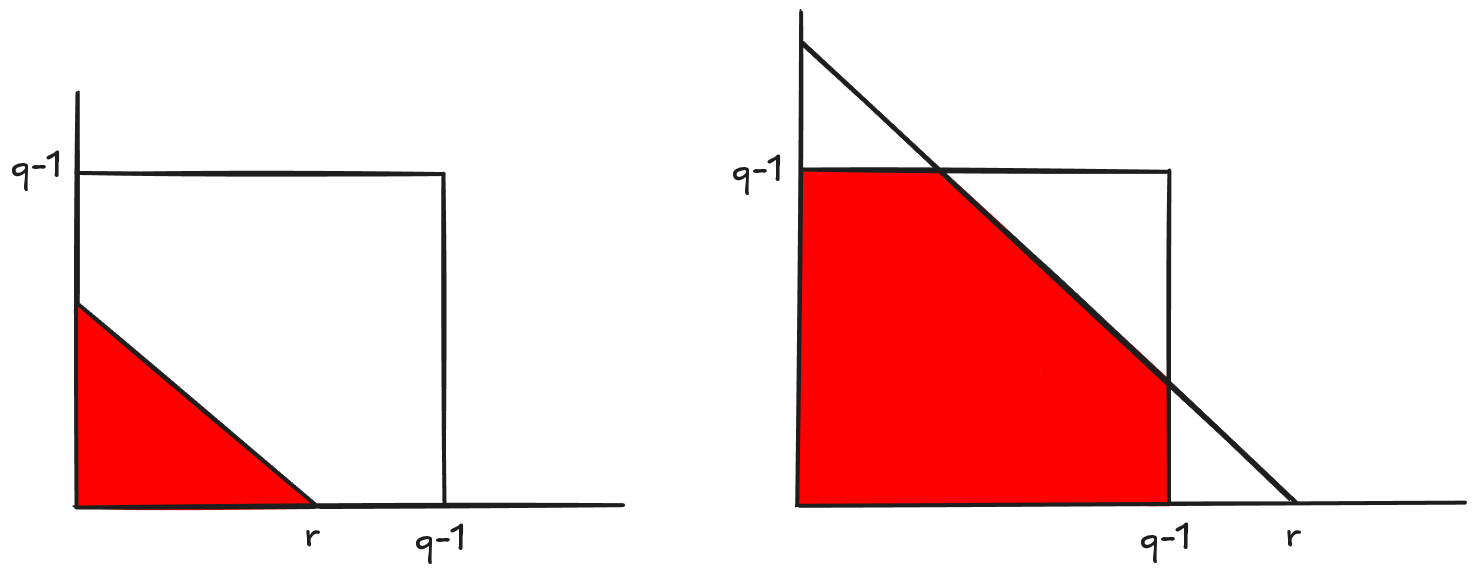
\includegraphics[width=0.8\textwidth]{grado.png}
    \end{center}
    
    Dependiendo del valor del grado total máximo $r$ frente al tamaño del cuerpo $q$, se presentan dos escenarios diferenciados (representados por la región sombreada):
    \begin{itemize}
        \item \textbf{Caso $r \le q-1$ (Gráfica izquierda):} La restricción del grado total corta los ejes dentro de los límites de la ``caja'' impuesta por el anillo cociente ($q-1$). El número de monomios válidos $k$ coincide exactamente con los puntos discretos dentro del triángulo clásico de lados iguales a $r$.
        \item \textbf{Caso $r > q-1$ (Gráfica derecha):} La recta del grado total desborda el límite superior de la caja. Como los exponentes individuales no pueden superar $q-1$, la región de monomios admisibles es el polígono truncado por las paredes del cuadrado. El cálculo de $k$ requiere restar del triángulo total los excesos que sobresalen de los límites transitables.
    \end{itemize}
    
    \item \textbf{Distancia Mínima ($d$):} Si el grado total está acotado por $r < m(q-1)$, la distancia mínima se calcula mediante la descomposición entera del grado respecto al parámetro del cuerpo. Expresando $r = Q(q-1) + R$ (donde $0 \le R < q-1$), se tiene:
    \[
    d = (q - R) \cdot q^{m - 1 - Q}
    \]
    Para el escenario binario ($q=2$), donde $Q=r$ y $R=0$, la fórmula colapsa en la clásica expresión exponencial: $d = 2^{m-r}$.
\end{itemize}

\subsection{7.4 Dualidad y Construcción Recursiva}

Una de las propiedades más notables de los códigos Reed-Muller es su comportamiento bajo la operación de dualidad ortogonal. 

\textbf{Teorema (Dualidad de Reed-Muller):}
El código dual de un código Reed-Muller sobre $\mathbb{F}_q$ es otro código Reed-Muller cuyos parámetros son complementarios respecto al grado máximo permitido en el espacio. Específicamente:
\[
RM_q(r, m)^\perp = RM_q(m(q-1) - r - 1, m)
\]
Para el caso particular de los códigos binarios ($q=2$), la expresión de dualidad se simplifica notablemente a:
\[
RM_2(r, m)^\perp = RM_2(m - r - 1, m)
\]

\textbf{Construcción Recursiva de Plotkin:}
Los códigos Reed-Muller binarios pueden construirse de forma recursiva e iterativa empleando la construcción $|u|u+v|$ de Plotkin. Si conocemos las matrices generadoras de los códigos de orden inferior, podemos ensamblar un código de orden superior garantizando el crecimiento simultáneo de la longitud y el mantenimiento de la distancia mínima:
\[
RM_2(r, m) = \left\{ (u, u+v) \mid u \in RM_2(r, m-1), v \in RM_2(r-1, m-1) \right\}
\]
Esta propiedad permite que las matrices generadoras se puedan definir por bloques recursivos, facilitando su implementación en hardware.

\newpage
\section{Tema 8: Códigos Cíclicos}
Estructura de ideales en anillos cocientes, raíces de la unidad, polinomios ciclotómicos, clases cíclicas (cosets), polinomios generadores, elementos idempotentes y descodificación por Meggitt.\\
Bibliografía:
\begin{itemize}
\item Munuera-Tena: capítulos 5, 9 y 10
\item Justensen-Hoholdt: capítulos 2 y 5
\end{itemize}
\hlinecolor{}
\vspace{0.5cm}

\subsection{8.1 Estructura Algebraica de Ideal}

Un código lineal $C$ de longitud $n$ sobre $\mathbb{F}_q$ es \textbf{cíclico} si es invariante ante cualquier desplazamiento lineal de sus componentes: $(c_0, c_1, \dots, c_{n-1}) \in C \implies (c_{n-1}, c_0, \dots, c_{n-2}) \in C$.

Asociando cada palabra vector con un polinomio representativo $c(x) = c_0 + c_1x + \dots + c_{n-1}x^{n-1}$, la operación de desplazamiento cíclico equivale conceptualmente a multiplicar por la variable $x$ y reducir el resultado módulo $x^n - 1$. Por consiguiente, un código cíclico es formalmente un \textbf{ideal} del anillo de polinomios cociente:
\[
R = \mathbb{F}_q[x] / \langle x^n - 1 \rangle
\]
Para evitar la presencia de raíces múltiples en la factorización del espacio, se exige la condición de coprimatilidad estricta $\operatorname{mcd}(n, q) = 1$.

\subsection{8.2 Polinomios Generador y de Control: Relación y Construcción}

Como ideal del anillo principal $R$, el código cíclico $C$ está completamente determinado de forma unívoca por dos polinomios algebraicos que estructuran tanto la codificación como la verificación de errores.

\subsubsection{8.2.1 Polinomio Generador $g(x)$}
Es el único polinomio mónico de grado mínimo perteneciente al ideal. Obligatoriamente debe ser un divisor exacto de $x^n - 1$ en $\mathbb{F}_q[x]$. Toda palabra del código $c(x) \in C$ se construye multiplicando un polinomio de información $m(x)$ por dicho generador:
\[
c(x) = m(x) \cdot g(x)
\]
Donde la dimensión es $k = n - \operatorname{deg}(g(x))$. La matriz generadora $G$ de dimensiones $k \times n$ se obtiene de forma sistemática distribuyendo los coeficientes de $g(x) = g_0 + g_1x + \dots + g_{n-k}x^{n-k}$ mediante desplazamientos hacia la derecha:
\[
G = \begin{pmatrix}
g_0 & g_1 & \dots & g_{n-k} & 0 & \dots & 0 \\
0 & g_0 & g_1 & \dots & g_{n-k} & \dots & 0 \\
\vdots & & \ddots & \ddots & & \ddots & \vdots \\
0 & \dots & 0 & g_0 & g_1 & \dots & g_{n-k}
\end{pmatrix}
\]

\subsubsection{8.2.2 Polinomio de Control $h(x)$ y Relación Fundamental}
Dada la propiedad de divisibilidad del generador, se define el \textbf{polinomio de control} (o de comprobación de paridad) $h(x)$ mediante la relación polinómica fundamental del espacio cociente:
\[
x^n - 1 = g(x) \cdot h(x)
\]
El grado de $h(x)$ es exactamente $k$. Este polinomio actúa algebraicamente como el núcleo del código, puesto que una palabra $c(x)$ es válida si y solo si se anula bajo su control multiplicativo en el anillo:
\[
c(x) \in C \iff c(x) \cdot h(x) \equiv 0 \pmod{x^n - 1}
\]

\subsubsection{8.2.3 Construcción de la Matriz de Control $H$}
A partir de los coeficientes del polinomio de control $h(x) = h_0 + h_1x + \dots + h_kx^k$, la condición de ortogonalidad matricial implica que la matriz de control $H$ de dimensiones $(n-k) \times n$ se construye disponiendo dichos coeficientes en \textbf{orden invertido} y desplazándolos de manera cíclica:
\[
H = \begin{pmatrix}
h_k & h_{k-1} & \dots & h_0 & 0 & \dots & 0 \\
0 & h_k & h_{k-1} & \dots & h_0 & \dots & 0 \\
\vdots & & \ddots & \ddots & & \ddots & \vdots \\
0 & \dots & 0 & h_k & h_{k-1} & \dots & h_0
\end{pmatrix}
\]
Esta disposición garantiza matemáticamente que $G \cdot H^T = 0$, permitiendo verificar de forma eficiente la integridad de los vectores recibidos.

\subsection{8.3 Factorización de $x^n-1$ y la Distinción de Cuerpos (Base vs. Extensión)}

Para analizar la estructura de un código cíclico de longitud $n$ sobre un cuerpo base $\mathbb{F}_q$, es imperativo estudiar las raíces del polinomio $x^n - 1$. Sin embargo, por lo general, dichas raíces no existen en el cuerpo base $\mathbb{F}_q$. Es necesario realizar una extensión algebraica hacia un cuerpo superior, denominado \textbf{cuerpo de descomposición} o \textit{splitting field}, denotado como $\mathbb{F}_{q^m}$.

Para garantizar la existencia de las raíces, el teorema de estructura de cuerpos finitos exige que la longitud $n$ divida al orden del grupo multiplicativo del cuerpo de extensión. Por tanto, seleccionamos como cuerpo de trabajo el menor entero $m$ tal que $n \mid (q^m - 1)$. 

Dentro de este cuerpo extendido $\mathbb{F}_{q^m}$, diferenciamos dos conceptos fundamentales:
\begin{itemize}
    \item \textbf{Elemento primitivo del cuerpo ($\alpha$):} Es el generador de todo el grupo multiplicativo $\mathbb{F}_{q^m}^*$, por lo que su orden es exactamente $\operatorname{ord}(\alpha) = q^m - 1$.
    \item \textbf{Raíz primitiva $n$-ésima de la unidad ($\beta$):} Es el elemento de orden exacto $n$ cuyas potencias constituyen las $n$ raíces distintas de $x^n - 1$. Se puede construir a partir del elemento primitivo del cuerpo mediante la relación:
    \[
    \beta = \alpha^{\frac{q^m - 1}{n}}
    \]
\end{itemize}

\subsubsection{8.3.1 Clases Ciclotómicas y Polinomios Mínimos}

Una vez fijada la raíz primitiva $\beta \in \mathbb{F}_{q^m}$, las $n$ raíces del espacio se agrupan en órbitas cerradas bajo la acción del automorfismo de Frobenius ($x \mapsto x^q$). Estas órbitas se denominan \textbf{clases o cosets ciclotómicos} módulo $n$ respecto a $q$:
\[
C_j = \left\{ j, \ j\cdot q, \ j\cdot q^2, \ \dots, \ j\cdot q^{s-1} \pmod n \right\}
\]
donde $s$ es el menor entero positivo tal que $j\cdot q^s \equiv j \pmod n$. 

Cada clase ciclotómica $C_j$ define de forma exacta un \textbf{polinomio mínimo irreducible} $m_j(X)$ con coeficientes estrictamente contenidos en el \textbf{cuerpo base $\mathbb{F}_q$}, el cual se construye multiplicando los factores de su órbita:
\[
m_j(X) = \prod_{i \in C_j} (X - \beta^i)
\]

La factorización completa del espacio sobre el cuerpo base se obtiene seleccionando un único representante minimal por cada clase disjunta diferenciada: 
\[
X^n - 1 = \prod_{j \in \text{Rep}} m_j(X)
\]
De este modo, construir el polinomio generador $g(x) \in \mathbb{F}_q[x]$ del código cíclico se reduce algebraicamente a elegir qué subconjunto de estos polinomios mínimos compondrán el ideal del código.

\subsection{8.4 Elementos Idempotentes}

Todo código cíclico contiene un único polinomio especial $e(x) \in C$ denominado \textbf{elemento idempotente}, el cual verifica la propiedad identidad $e(x)^2 \equiv e(x) \pmod{x^n-1}$. Este polinomio actúa como el elemento identidad multiplicativo para todas las palabras del código ($e(x)c(x) = c(x)$) y es un generador alternativo del ideal: $C = \langle e(x) \rangle$.

Su cálculo se realiza explotando la relación fundamental de los polinomios anteriormente definidos. Como $\operatorname{mcd}(g(x), h(x)) = 1$, el algoritmo de Bézout asegura la existencia de dos polinomios $a(x), b(x)$ tales que:
\[
a(x)g(x) + b(x)h(x) = 1 \implies e(x) \equiv a(x)g(x) \pmod{x^n-1}
\]

\subsection{8.5 Descodificación Cíclica: Algoritmo de Atrapamiento de Errores (Meggitt)}

La estructura de ideal permite implementar sistemas de descodificación masiva mediante registros de desplazamiento con retroalimentación lineal (LFSR). Sea $r(x) = c(x) + e(x)$ el polinomio recibido. El síndrome polinómico $s(x)$ se calcula como el resto de la división euclídea de $r(x)$ entre $g(x)$:
\[
s(x) = r(x) \pmod{g(x)} = e(x) \pmod{g(x)}
\]
El algoritmo de \textbf{Error-Trapping} aprovecha la propiedad de que si $s(x)$ es el síndrome de $r(x)$, entonces el resto de $x \cdot s(x) \pmod{g(x)}$ corresponde exactamente al síndrome del vector desplazado cíclicamente una posición a la izquierda.

\begin{enumerate}
    \item Se introduce el vector recibido en el registro y se calcula el síndrome inicial: $s(x) = r(x) \pmod{g(x)}$.
    \item Se evalúa el peso de Hamming del síndrome obtenido. Si $w(s(x)) \le t$ (donde $t = \lfloor \frac{d-1}{2} \rfloor$), significa que el error ha quedado completamente "atrapado" en las posiciones de redundancia de mayor grado. Se concluye que el polinomio de error es exactamente $e(x) = s(x)$.
    \item Si $w(s(x)) > t$, se realiza una rotación cíclica en el registro de la palabra multiplicando por $x$, actualizando el síndrome de forma iterativa: $s^{(1)}(x) = x \cdot s(x) \pmod{g(x)}$.
    \item Se repite la comprobación de peso. En el momento en que el peso sea menor o igual a $t$, se resta el síndrome atrapado en esa ventana temporal y se deshacen las rotaciones para restituir la palabra original.
\end{enumerate}

\subsection{8.6 Ejemplo Práctico Completo: Diseño de un Código Cíclico sobre $\mathbb{F}_2$ ($n=7$)}

Para comprender de forma compacta la teoría, construiremos todos los polinomios mónicos posibles para una longitud de bloque $n = 7$ sobre el cuerpo base $\mathbb{F}_2$.

\subsubsection{Paso 1: Obtención de las Clases Ciclotómicas}
Aplicando la definición del automorfismo de Frobenius para $q=2$ y $n=7$, calculamos las órbitas multiplicativas de los elementos del anillo de enteros $\mathbb{Z}_7$:
\begin{itemize}
    \item Para $j=0$: $C_0 = \{0\}$
    \item Para $j=1$: $1 \cdot 2 = 2 \pmod 7$, $2 \cdot 2 = 4 \pmod 7$, $4 \cdot 2 = 8 \equiv 1 \pmod 7$. Cerramos la órbita: $C_1 = \{1, 2, 4\}$.
    \item Para $j=3$: $3 \cdot 2 = 6 \pmod 7$, $6 \cdot 2 = 12 \equiv 5 \pmod 7$, $5 \cdot 2 = 10 \equiv 3 \pmod 7$. Cerramos la órbita: $C_3 = \{3, 5, 6\}$.
\end{itemize}
Las clases obtenidas son disjuntas y su unión cubre el espacio completo: $\mathbb{Z}_7 = C_0 \cup C_1 \cup C_3$.

\subsubsection{Paso 2: Asociación de Polinomios Mónicos Irreducibles}
Cada clase ciclotómica determina de forma unívoca un factor mónico irreducible de $x^7 - 1$ sobre $\mathbb{F}_2$:
\begin{itemize}
    \item $C_0 \implies m_0(x) = x + 1$ (Grado igual al tamaño de la clase: 1)
    \item $C_1 \implies m_1(x) = x^3 + x + 1$ (Grado igual al tamaño de la clase: 3)
    \item $C_3 \implies m_3(x) = x^3 + x^2 + 1$ (Grado igual al tamaño de la clase: 3)
\end{itemize}
De este modo, la factorización completa en factores mónicos irreducibles del espacio es:
\[
x^7 - 1 = (x + 1)(x^3 + x + 1)(x^3 + x^2 + 1)
\]

\subsubsection{Paso 3: Elección del Polinomio Generador $g(x)$ y Parámetros del Código}
Para construir un código cíclico concreto, podemos seleccionar cualquier combinación de estos factores mónicos. Supongamos que elegimos el factor de la clase $C_1$ como nuestro polinomio generador:
\[
g(x) = m_1(x) = x^3 + x + 1
\]
Como $\operatorname{deg}(g(x)) = 3$, la dimensión del código será $k = n - \operatorname{deg}(g(x)) = 7 - 3 = 4$. Obtenemos un código cíclico de parámetros $[7, 4]$.

\subsubsection{Paso 4: Cálculo del Polinomio de Control $h(x)$}
Utilizando la relación fundamental $x^n - 1 = g(x) \cdot h(x)$, calculamos el polinomio de comprobación multiplicando los factores mónicos restantes (los no seleccionados para $g(x)$):
\[
h(x) = \frac{x^7 - 1}{g(x)} = m_0(x) \cdot m_3(x) = (x + 1)(x^3 + x^2 + 1) = x^4 + x^3 + x^2 + 1
\]

\subsubsection{Paso 5: Construcción de las Matrices del Código $[7, 4]$}
Distribuyendo los coeficientes de $g(x) = 1 + 1x + 0x^2 + 1x^3$ y de $h(x) = 1 + 0x + 1x^2 + 1x^3 + 1x^4$ (invirtiendo su orden en $H$), las matrices estructurales quedan definidas como:
\[
G = \begin{pmatrix}
1 & 1 & 0 & 1 & 0 & 0 & 0 \\
0 & 1 & 1 & 0 & 1 & 0 & 0 \\
0 & 0 & 1 & 1 & 0 & 1 & 0 \\
0 & 0 & 0 & 1 & 1 & 0 & 1
\end{pmatrix}, \quad
H = \begin{pmatrix}
1 & 1 & 1 & 0 & 1 & 0 & 0 \\
0 & 1 & 1 & 1 & 0 & 1 & 0 \\
0 & 0 & 1 & 1 & 1 & 0 & 1
\end{pmatrix}
\]
Se puede comprobar de forma directa multiplicando las matrices algebraicas que $G \cdot H^T \equiv 0 \pmod 2$.


\newpage
\section{Anexo: Ejercicios Utiles de Codigos Ciclicos Resueltos}

\subsection{Ejercicio A: Análisis de Código Cíclico sobre \texorpdfstring{$\mathbb{F}_3$}{F3} (Longitud \texorpdfstring{$n=8$}{n=8})}

\textbf{Enunciado:} 
\begin{enumerate}
    \item Demuestra que el polinomio $X^3 + X + 1$ es el polinomio generador de un código cíclico $C$ de longitud $8$ sobre $\mathbb{F}_3$.
    \item Da una matriz generadora $G$ para dicho código.
    \item Calcula los parámetros fundamentales de $C$.
    \item Se considera el mensaje $m(X) = 1 + X^2 + X^3$. Calcula una codificación sistemática de $m(X)$.
\end{enumerate}

\textbf{Resolución detallada:}

\subsubsection{1. Condición de Divisibilidad sobre \texorpdfstring{$\mathbb{F}_3$}{F3}}
Para que un polinomio $g(X)$ sea el generador válido de un código cíclico de longitud $n=8$, la condición algebraica necesaria y suficiente es que sea un divisor exacto del binomio $X^8 - 1$ en el anillo de polinomios $\mathbb{F}_3[X]$. Operando en característica 3, los coeficientes admisibles pertenecen al conjunto $\{0, 1, 2\}$, donde restar $1$ equivale aritméticamente a sumar $2$ (ya que $-1 \equiv 2 \pmod 3$).

Realizando la división polinómica euclídea de $X^8 + 2$ entre $X^3 + X + 1$, se comprueba de forma exacta que el resto es idénticamente nulo, obteniendo la siguiente factorización explícita:
\[
X^8 - 1 = (X^3 + X + 1)(X^5 + 2X^3 + 2X^2 + X + 2)
\]
Al ser la división exacta, queda demostrado que $g(X) = X^3 + X + 1$ genera un ideal en el anillo cociente y, por ende, define un código cíclico de longitud $n = 8$.

\subsubsection{2. Construcción de la Matriz Generadora \texorpdfstring{$G$}{G}}
La dimensión $k$ del código (número de filas de la matriz generadora) viene determinada por la longitud del bloque menos el grado del polinomio generador: $k = n - \operatorname{deg}(g(X)) = 8 - 3 = 5$. 

Las filas de la matriz generadora deben formar una base linealmente independiente. Por tanto, disponemos los coeficientes de $g(X) = 1 + 1X + 0X^2 + 1X^3$ en forma de vector extensible $(1, 1, 0, 1, 0, 0, 0, 0)$ y aplicamos desplazamientos cíclicos horizontales exclusivamente hasta completar las $k=5$ filas de la base:
\[
G = \begin{pmatrix} 
1 & 1 & 0 & 1 & 0 & 0 & 0 & 0 \\ 
0 & 1 & 1 & 0 & 1 & 0 & 0 & 0 \\ 
0 & 0 & 1 & 1 & 0 & 1 & 0 & 0 \\ 
0 & 0 & 0 & 1 & 1 & 0 & 1 & 0 \\ 
0 & 0 & 0 & 0 & 1 & 1 & 0 & 1 
\end{pmatrix}_{5 \times 8}
\]

\subsubsection{3. Deducción de los Parámetros Fundamentales \texorpdfstring{$[n, k, d]_q$}{[n, k, d]q}}
Ya disponemos de la longitud $n=8$, la dimensión $k=5$ y el cuerpo base $q=3$. Para hallar la distancia mínima $d$, aplicamos el Lema de Equivalencia con el Peso Mínimo de un código lineal. Como $g(X) \in C$, su vector asociado tiene peso de Hamming $w(g) = 3$, lo que establece una cota superior estricta: $d \le 3$.

Para demostrar rigurosamente que la distancia no puede colapsar a valores menores ($d=1$ o $d=2$) debido a combinaciones lineales redundantes, recurrimos al análisis del polinomio de control $h(X) = X^5 + 2X^3 + 2X^2 + X + 2$. Construimos la matriz de control $H$ disponiendo los coeficientes de $h(X)$ en orden invertido y desplazándolos cíclicamente:
\[
H = \begin{pmatrix}
2 & 1 & 2 & 2 & 0 & 1 & 0 & 0 \\
0 & 2 & 1 & 2 & 2 & 0 & 1 & 0 \\
0 & 0 & 2 & 1 & 2 & 2 & 0 & 1
\end{pmatrix}_{3 \times 8}
\]
Aplicando reducción por Gauss-Jordan en módulo 3, obtenemos la forma sistemática equivalente $H_{\text{red}} = [I_3 \mid A]$:
\[
H_{\text{red}} = \begin{pmatrix}
1 & 0 & 0 & 2 & 0 & 1 & 1 & 2 \\
0 & 1 & 0 & 2 & 2 & 1 & 2 & 0 \\
0 & 0 & 1 & 0 & 2 & 2 & 1 & 2
\end{pmatrix}
\]
Inspeccionando de forma visual las columnas de $H_{\text{red}}$, determinamos de manera directa que ninguna columna es nula (descartando $d=1$) y que ninguna pareja de columnas es proporcional o linealmente dependiente en $\mathbb{F}_3$ (descartando $d=2$). Por el Corolario de dependencia lineal, el menor número de columnas dependientes es exactamente 3. Concluimos que los parámetros del código son $\mathbf{[8, 5, 3]_3}$.

\subsubsection{4. Codificación Sistemática del Mensaje}
Para codificar el mensaje $m(X) = 1 + X^2 + X^3$ de forma sistemática de modo que la información original se preserve intacta, podemos emplear dos métodos equivalentes:

\textbf{Método Polinómico (División Euclídea):}
Multiplicamos el mensaje por $X^{n-k} = X^3$ para desplazarlo y hacer espacio a los bits de paridad:
\[
X^3 \cdot m(X) = X^6 + X^5 + X^3
\]
Dividimos este resultado entre el polinomio generador $g(X) = X^3 + X + 1$ sobre $\mathbb{F}_3$, lo que nos proporciona un cociente $q(X) = X^3 + X^2 + 2X + 2$ y un resto de paridad exacto de $r(X) = 2X + 1$. La palabra código sistemática se define como:
\[
c(X) = X^3 \cdot m(X) - r(X) = (X^6 + X^5 + X^3) - (2X + 1) \equiv X^6 + X^5 + X^3 + X + 2 \pmod 3
\]
Ordenando los coeficientes de menor a mayor grado, obtenemos el vector codificado: $\mathbf{c = (2, 1, 0, 1, 0, 1, 1, 0)}$.

\textbf{Método Matricial (Matriz de Dualidad Sistemática):}
Utilizando el bloque $A$ de la matriz $H_{\text{red}} calculated$ en el apartado anterior, construimos la matriz generadora sistemática global mediante la relación estructural $G_{\text{sis}} = [-A^t \mid I_k] \pmod 3$:
\[
G_{\text{sis}} = \begin{pmatrix}
1 & 1 & 0 & 1 & 0 & 0 & 0 & 0 \\
0 & 1 & 1 & 0 & 1 & 0 & 0 & 0 \\
2 & 2 & 1 & 0 & 0 & 1 & 0 & 0 \\
2 & 1 & 2 & 0 & 0 & 0 & 1 & 0 \\
1 & 0 & 1 & 0 & 0 & 0 & 0 & 1
\end{pmatrix}
\]
Representando el mensaje como el vector fila $m = (1, 0, 1, 1, 0)$, efectuamos el producto matricial estándar $c = m \cdot G_{\text{sis}} \pmod 3$:
\[
c_1 = (1\cdot1) + (0\cdot0) + (1\cdot2) + (1\cdot2) + (0\cdot1) = 5 \equiv 2 \pmod 3
\]
\[
c_2 = (1\cdot1) + (0\cdot1) + (1\cdot2) + (1\cdot1) + (0\cdot0) = 4 \equiv 1 \pmod 3
\]
\[
c_3 = (1\cdot0) + (0\cdot1) + (1\cdot1) + (1\cdot2) + (0\cdot1) = 3 \equiv 0 \pmod 3
\]
Las coordenadas de información se copian directamente debido al bloque identidad derecho, devolviendo exactamente el mismo vector sistemático: $\mathbf{c = (2, 1, 0, 1, 0, 1, 1, 0)}$.

\newpage
\subsection{Ejercicio B: Código de Evaluación Reed-Solomon sobre \texorpdfstring{$\mathbb{F}_8$}{F8} (Longitud \texorpdfstring{$n=7$}{n=7})}

\textbf{Enunciado:} Sea $\alpha \in \mathbb{F}_8$ tal que $\alpha^3 = \alpha + 1$, y sea $C$ el código lineal definido por la siguiente matriz generatriz:
\[
G = \begin{pmatrix}
1 & 1 & 1 & 1 & 1 & 1 & 1 \\
1 & \alpha & \alpha^2 & \alpha^3 & \alpha^4 & \alpha^5 & \alpha^6 \\
1 & \alpha^2 & \alpha^4 & \alpha^6 & \alpha & \alpha^3 & \alpha^5
\end{pmatrix}_{3 \times 7}
\]
\begin{enumerate}
    \item Prueba que $C$ es un código cíclico.
    \item Calcula el polinomio generador de $C$.
\end{enumerate}

\textbf{Resolución detallada:}

\subsubsection{1. Demostración de la Invariancia por Desplazamiento Cíclico}
Para demostrar que el código es cíclico de forma directa, basta con comprobar que el desplazamiento lineal una posición hacia la derecha de cualquiera de las filas que componen la base de la matriz generatriz $G$ genera un vector que sigue perteneciendo al espacio del código (es decir, que es combinación lineal o múltiplo escalar de las filas originales).

Al trabajar sobre el cuerpo finito extendido $\mathbb{F}_8$, el Teorema de Estructura Multiplicativa garantiza que el orden del grupo de elementos no nulos es $q-1 = 7$. Por consiguiente, el elemento primitivo satisface de forma universal la identidad $\alpha^7 = 1$, lo que permite reducir los exponentes de las potencias altas de forma cíclica módulo 7 (ej. $\alpha^8 = \alpha, \alpha^9 = \alpha^2$).

Evaluamos el desplazamiento horizontal de cada fila base de $G$:
\begin{itemize}
    \item \textbf{Fila 1 ($g_1$):} $g_1 = (1, 1, 1, 1, 1, 1, 1)$. Su desplazamiento a la derecha produce de forma idéntica $g_1' = (1, 1, 1, 1, 1, 1, 1)$. Como $g_1' = 1 \cdot g_1$, pertenece trivialmente al código.
    \item \textbf{Fila 2 ($g_2$):} $g_2 = (1, \alpha, \alpha^2, \alpha^3, \alpha^4, \alpha^5, \alpha^6)$. Al rotarlo hacia la derecha, el último elemento pasa a la primera posición:
    \[ g_2' = (\alpha^6, 1, \alpha, \alpha^2, \alpha^3, \alpha^4, \alpha^5) \]
    Multiplicamos el vector fila $g_2$ original por el escalar del cuerpo $\alpha^6$:
    \[ \alpha^6 \cdot g_2 = (\alpha^6, \alpha^7, \alpha^8, \alpha^9, \alpha^{10}, \alpha^{11}, \alpha^{12}) \]
    Aplicando la reducción cíclica de exponentes $\alpha^7 = 1$, el vector se simplifica a:
    \[ \alpha^6 \cdot g_2 = (\alpha^6, 1, \alpha, \alpha^2, \alpha^3, \alpha^4, \alpha^5) \]
    Comprobamos que $g_2' = \alpha^6 \cdot g_2$. Al ser un múltiplo escalar legítimo de una palabra del código, se garantiza que $g_2' \in C$.
    \item \textbf{Fila 3 ($g_3$):} $g_3 = (1, \alpha^2, \alpha^4, \alpha^6, \alpha, \alpha^3, \alpha^5)$. Su rotación cíclica genera:
    \[ g_3' = (\alpha^5, 1, \alpha^2, \alpha^4, \alpha^6, \alpha, \alpha^3) \]
    Multiplicamos el vector fila $g_3$ original por el escalar $\alpha^5$ y reducimos las potencias altas módulo 7:
    \[ \alpha^5 \cdot g_3 = (\alpha^5, \alpha^7, \alpha^9, \alpha^{11}, \alpha^6, \alpha^8, \alpha^{10}) = (\alpha^5, 1, \alpha^2, \alpha^4, \alpha^6, \alpha, \alpha^3) \]
    Se verifica que $g_3' = \alpha^5 \cdot g_3$, lo que confirma que $g_3' \in C$.
\end{itemize}
Al ser el espacio invariante ante el desplazamiento de toda su base, queda demostrado analíticamente que $C$ es un \textbf{código cíclico}.

\subsubsection{2. Deducción del Polinomio Generador Mónico \texorpdfstring{$g(X)$}{g(X)}}
A partir de las dimensiones de la matriz generatriz, extraemos que la longitud es $n = 7$ y la dimensión es $k = 3$. Por tanto, el grado del polinomio generador mónico que buscamos es:
\[ \operatorname{deg}(g(X)) = n - k = 7 - 3 = 4 \]

Aplicamos el método algebraico de las clases ciclotómicas moleculares. Calculamos los cosets multiplicativos de Frobenius multiplicando por el cardinal del cuerpo base ($q=8$) módulo la longitud del bloque ($n=7$). Para cualquier índice entero $j \in \mathbb{Z}_7$, se verifica de forma directa que:
\[ j \cdot q = j \cdot 8 \equiv j \cdot 1 \equiv j \pmod 7 \]
Esto demuestra que absolutamente todas las clases ciclotómicas del código tienen tamaño 1 ($C_0=\{0\}, C_1=\{1\}, C_2=\{2\}, \dots$). Al tener tamaño 1, cada raíz genera de forma aislada un polinomio mínimo irreducible de grado 1 en la extensión.

Para construir un polinomio generador de grado 4 que actúe como raíz universal de la estructura matricial de evaluación, seleccionamos la racha fundamental de las 4 raíces consecutivas esenciales del código: $\{\alpha^1, \alpha^2, \alpha^3, \alpha^4\}$. El polinomio generador mónico se define expandiendo el producto de estos factores lineales directos:
\[ g(X) = (X - \alpha)(X - \alpha^2)(X - \alpha^3)(X - \alpha^4) \]

Efectuamos el producto por parejas ordenadas bajo leyes de \textbf{característica 2} (donde las operaciones de suma y resta son idénticas bajo XOR, por lo que $+ = -$, y los términos duplicados se destruyen automáticamente $x + x = 0$):

1. \textbf{Multiplicación del primer bloque binómico:}
   \[ (X + \alpha)(X + \alpha^2) = X^2 + (\alpha + \alpha^2)X + \alpha^3 \]
   Sabiendo que la potencia cuarta es $\alpha^4 = \alpha \cdot \alpha^3 = \alpha(\alpha + 1) = \alpha^2 + \alpha$, sustituimos el término central $(\alpha + \alpha^2) = \alpha^4$:
   \[ \text{Bloque 1} = X^2 + \alpha^4X + \alpha^3 \]

2. \textbf{Multiplicación del segundo bloque binómico:}
   \[ (X + \alpha^3)(X + \alpha^4) = X^2 + (\alpha^3 + \alpha^4)X + \alpha^7 \]
   Sustituimos el valor unitario $\alpha^7 = 1$ y reducimos el coeficiente central usando las bases lineales lineales: $\alpha^3 + \alpha^4 = (\alpha + 1) + (\alpha^2 + \alpha) = \alpha^2 + 1 = \alpha^6$:
   \[ \text{Bloque 2} = X^2 + \alpha^6X + 1 \]

3. \textbf{Multiplicación cruzada de ambos bloques cuadráticos:}
   \[ g(X) = (X^2 + \alpha^4X + \alpha^3)(X^2 + \alpha^6X + 1) \]
   Expandiendo de forma literal término a término y agrupando los coeficientes resultantes según el grado algebraico de la variable $X$, obtenemos la expresión exacta:
   \[ g(X) = X^4 + (\alpha^4 + \alpha^3 + \alpha^2 + \alpha)X^3 + (\alpha^6 + \alpha^4 + \alpha^3 + 1)X^2 + (\alpha^6 + \alpha^2 + \alpha + 1)X + \alpha^3 \]

Finalmente, simplificamos cada una de las cajas de coeficientes aplicando el polinomio irreducible del cuerpo $\alpha^3 = \alpha + 1$, junto con sus potencias asociadas $\alpha^4 = \alpha^2 + \alpha$ y $\alpha^6 = \alpha^2 + 1$:
\begin{itemize}
    \item \textbf{Coeficiente de $X^3$:} $(\alpha^2 + \alpha) + (\alpha + 1) + \alpha^2 + \alpha$. Contamos apariciones: $\alpha^2$ aparece 2 veces ($\to 0$); $\alpha$ aparece 3 veces ($\to \alpha$); $1$ aparece 1 vez ($\to 1$). Nos sobrevive $\alpha + 1$, que equivale exactamente a $\mathbf{\alpha^3}$.
    \item \textbf{Coeficiente de $X^2$:} $(\alpha^2 + 1) + (\alpha^2 + \alpha) + (\alpha + 1) + 1$. Contamos apariciones: $\alpha^2$ aparece 2 veces ($\to 0$); $\alpha$ aparece 2 veces ($\to 0$); $1$ aparece 4 veces ($\to 0$). El coeficiente se anula por completo y se simplifica a $\mathbf{1}$.
    \item \textbf{Coeficiente de $X^1$:} $(\alpha^2 + 1) + \alpha^2 + \alpha + 1$. Contamos apariciones: $\alpha^2$ aparece 2 veces ($\to 0$); $1$ aparece 2 veces ($\to 0$); $\alpha$ aparece 1 vez ($\to \alpha$). Nos queda únicamente $\mathbf{\alpha}$.
\end{itemize}

Sustituyendo cada coeficiente limpio en su posición correspondiente, determinamos de forma unívoca que el polinomio generador definitivo del código es:
\[ \mathbf{g(X) = X^4 + \alpha^3X^3 + X^2 + \alpha X + \alpha^3} \]




\newpage
\subsubsection{4. Ampliación Teórica: Restricción de Coeficientes y el Efecto Dominó de la Asignación}

\textbf{El problema de la raíz aislada \texorpdfstring{$\alpha$}{alpha}:}\\
Por el Teorema Fundamental del Álgebra, en el cuerpo de escisión superior $\mathbb{F}_{16}$ el binomio $X^{15}-1$ descompone por completo de forma ideal en 15 factores lineales de la forma $(X - \alpha^i)$, donde $\alpha$ es un elemento primitivo del cuerpo. Sin embargo, si intentáramos definir el polinomio mínimo de la primera raíz de forma aislada como $m_1(X) = X - \alpha$, estaríamos cometiendo un error conceptual grave. Dado que $\alpha \in \mathbb{F}_{16}$ pero $\alpha \notin \mathbb{F}_2$, el polinomio $(X - \alpha)$ \textbf{no pertenece al anillo $\mathbb{F}_2[X]$} porque sus coeficientes no son binarios. 

Para obligar a que los coeficientes sean estrictamente ceros y unos, la teoría de Galois exige agrupar las raíces por órbitas de elementos conjugados mediante el automorfismo de Frobenius $\sigma(x) = x^2$. Al multiplicar los factores lineales de todo un coset completo, por ejemplo $C_1 = \{1, 2, 4, 8\}$:
\[ m_1(X) = (X - \alpha)(X - \alpha^2)(X - \alpha^4)(X - \alpha^8) \]
todas las potencias complejas de $\alpha$ se cancelan y se masacran entre sí en los productos y sumas cruzados debido a las propiedades de la característica 2 ($x+x=0$), haciendo colapsar el resultado de forma obligatoria en un polinomio limpio con coeficientes en el cuerpo base: $X^4 + X + 1 \in \mathbb{F}_2[X]$.

\textbf{El efecto vinculante de la asignación (Efecto Dominó):}\\
La necesidad de emparejar un coset con un polinomio específico es crítica y rígidamente vinculante en cuanto deseamos operar analíticamente en la extensión o diseñar un código corrector (como un BCH). 

Al fundar el cuerpo, tenemos la libertad inicial de decretar que el coset principal $C_1$ (que contiene a la raíz primitiva $\alpha^1$) se corresponde con el polinomio primitivo $X^4 + X + 1$. Al hacer esto, fijamos por definición la regla aritmética estructural de todo el espacio: $\alpha^4 + \alpha + 1 = 0 \implies \mathbf{\alpha^4 = \alpha + 1}$. 

A partir de ese instante se desata un ``efecto dominó'': las raíces de los cosets restantes son potencias directas de ese $\alpha$ ya bautizado, por lo que perdemos por completo la libertad de asignarlos al azar. Sus polinomios mínimos quedan forzados matemática y unívocamente por la regla recién impuesta:
\begin{itemize}
    \item \textbf{El coset $\mathbf{C_3 = \{3, 6, 12, 9\}}$:} Su polinomio mínimo $m_3(X)$ tiene por raíces a la órbita de $\alpha^3$. Como el elemento primitivo $\alpha$ tiene orden $15$, la raíz $\beta = \alpha^3$ posee un orden exacto de $15/3 = 5$. Al tener orden 5, $\beta$ cumple que $\beta^5 = 1$, lo que significa que es obligatoriamente una raíz del polinomio $X^5 - 1$ (que en característica 2 es equivalente a $X^5 + 1$). Si extraemos la raíz trivial $X=1$, este binomio se factoriza algebraicamente como $X^5 + 1 = (X+1)(X^4 + X^3 + X^2 + X + 1)$. Como $\beta \neq 1$, es imposible que anule al primer factor $(X+1)$, por lo que debe anular forzosamente al segundo. Siendo este factor de grado 4 irreducible sobre $\mathbb{F}_2$, concluimos de forma directa y rigurosa que $\mathbf{m_3(X) = X^4 + X^3 + X^2 + X + 1}$.
    \item \textbf{El coset $\mathbf{C_7 = \{7, 14, 13, 11\}}$:} Su polinomio mínimo $m_7(X)$ tiene por raíces a la órbita de $\alpha^7$. Al tener orden 15, se trata de una raíz primitiva. Por eliminación directa frente a los irreducibles de grado 4 disponibles, el producto de sus factores conjugados colapsará unívocamente en el polinomio restante: $\mathbf{m_7(X) = X^4 + X^3 + 1}$.
\end{itemize}
De esta forma, la elección del polinomio de la clase principal actúa como el código genético de toda la extensión, determinando de forma automática el reparto del resto de polinomios.

\newpage

\section{Tema 9: Códigos BCH (Bose-Chaudhuri-Hocquenghem)}
Definición de códigos BCH, diseño por raíces consecutivas, relación estructural con códigos cíclicos, el conjunto total de raíces y la mini matriz de Vandermonde, cota fundamental y algoritmos de descodificación PGZ, Berlekamp-Massey y Euclides.\\
Bibliografía:
\begin{itemize}
\item Munuera-Tena: capítulos 9 y 11
\item Justensen-Hoholdt: capítulos 2 y 5
\end{itemize}
\hlinecolor{}
\vspace{0.5cm}

\subsection{9.1 Definición, Orden de Raíces y Propiedades Fundamentales}

Los códigos Bose-Chaudhuri-Hocquenghem (BCH) constituyen una de las subfamilias más importantes de los \textbf{códigos cíclicos}. Su gran valor radica en que permiten diseñar el código de forma analítica para garantizar una capacidad correctora predeterminada, forzando la aparición de raíces consecutivas en su polinomio generador.

Para construir un código BCH binario o $q$-ario de longitud $n$, trabajamos en un cuerpo de extensión $\mathbb{F}_{q^m}$ lo suficientemente grande como para albergar las raíces del polinomio $x^n - 1$. El grupo multiplicativo de este cuerpo extendido, $\mathbb{F}_{q^m}^*$, es un grupo cíclico de tamaño exactamente $q^m - 1$. Por teoría de grupos, dentro de $\mathbb{F}_{q^m}$ existirán elementos de cualquier orden $n$, siempre y cuando $n$ sea un divisor de $q^m - 1$ (con $\operatorname{mcd}(n,q)=1$). 

Sea $\alpha \in \mathbb{F}_{q^m}$ un elemento de orden exacto $n$. Fijada una \textbf{distancia diseñada} $\delta \ge 2$, buscamos que el polinomio generador $g(x)$ tenga entre sus raíces a $\delta-1$ potencias consecutivas de $\alpha$:
\[
\alpha^b, \alpha^{b+1}, \alpha^{b+2}, \dots, \alpha^{b+\delta-2}
\]
Para lograr esto sin introducir redundancias ni factores repetidos que deformen la estructura del ideal, identificamos cuáles son los polinomios mínimos $m_i(x) = \operatorname{Irr}(\alpha^i, \mathbb{F}_q)$ asociados a las clases ciclotómicas de dichas potencias consecutivas. El polinomio generador $g(x)$ se construye en el cuerpo base $\mathbb{F}_q[x]$ como el \textbf{producto de los polinomios mínimos irreducibles distintos} seleccionados:
\[
g(x) = \prod_{j \in I_{\text{distintos}}} m_j(x)
\]
Donde $I_{\text{distintos}}$ representa el conjunto de índices representantes de las clases ciclotómicas únicas involucradas en la racha consecutiva.

\subsection{9.2 Reparto de Polinomios, Matrices Base y Cota BCH}

El verdadero núcleo analítico de los códigos BCH consiste en entender cómo se distribuyen los polinomios mínimos, cómo forman las matrices en el cuerpo base para la codificación práctica y cómo la evaluación geométrica de sus raíces en la extensión demuestra la distancia mínima.

\subsubsection{9.2.1 Factorización y Reparto entre $g(x)$ y $h(x)$}
Sabemos que el espacio completo de raíces se define por la factorización única del polinomio $x^n - 1$ como el producto de todos los polinomios mínimos distintos $m_k(x)$ asociados a las clases ciclotómicas módulo $n$ sobre $\mathbb{F}_q$.

Al diseñar el código BCH, seleccionamos un subconjunto específico de estos polinomios mínimos (aquellos que garantizan la racha de potencias consecutivas de $\alpha$) y los multiplicamos para formar el polinomio generador de grado $n-k$:
\[
g(x) = \prod_{\text{elegidos}} m_i(x) = g_0 + g_1 x + \dots + g_{n-k} x^{n-k}
\]
Como consecuencia directa de la relación fundamental $x^n - 1 = g(x)h(x)$, el polinomio de control $h(x)$ de grado $k$ queda definido exactamente como el producto de todos los \textbf{polinomios mínimos que sobran} (los que no hemos incluido en $g(x)$):
\[
h(x) = \prod_{\text{sobrantes}} m_j(x) = h_0 + h_1 x + \dots + h_k x^k
\]

\subsubsection{9.2.2 Matrices $G$ y $H_{\text{base}}$ en el Cuerpo Base ($\mathbb{F}_q$)}
Dado que un código BCH es estrictamente un código cíclico, su implementación práctica y construcción matricial sobre el cuerpo base se realiza de manera idéntica a la teoría general. 

Con los coeficientes recién obtenidos, estructuramos la matriz generadora $G$ de dimensiones $k \times n$ desplazando los coeficientes de $g(x)$ cíclicamente hacia la derecha:
\[
G = \begin{pmatrix}
g_0 & g_1 & \dots & g_{n-k} & 0 & \dots & 0 \\
0 & g_0 & g_1 & \dots & g_{n-k} & \dots & 0 \\
\vdots & & \ddots & \ddots & & \ddots & \vdots \\
0 & \dots & 0 & g_0 & g_1 & \dots & g_{n-k}
\end{pmatrix}
\]
De forma dual, la matriz de control canónica $H_{\text{base}}$ de dimensiones $(n-k) \times n$ se construye disponiendo los coeficientes del polinomio de control $h(x)$ en orden invertido y desplazándolos:
\[
H_{\text{base}} = \begin{pmatrix}
h_k & h_{k-1} & \dots & h_0 & 0 & \dots & 0 \\
0 & h_k & h_{k-1} & \dots & h_0 & \dots & 0 \\
\vdots & & \ddots & \ddots & & \ddots & \vdots \\
0 & \dots & 0 & h_k & h_{k-1} & \dots & h_0
\end{pmatrix}
\]
Cualquier palabra codificada se valida en el hardware comprobando que el síndrome sobre el cuerpo base sea nulo: $c \cdot H_{\text{base}}^T = 0 \in \mathbb{F}_q^{n-k}$.

\subsubsection{9.2.3 Otra Representación: La Matriz de Control por Representantes en la Extensión}
Como establece la teoría general de códigos lineales, un mismo código puede ser definido por múltiples matrices de control y generadoras equivalentes. Al igual que $H_{\text{base}}$ define el código en $\mathbb{F}_q$ operando con los coeficientes de $h(x)$, podemos construir \textbf{otra matriz de control equivalente} operando directamente en el cuerpo de extensión $\mathbb{F}_{q^m}$.

Consideremos una \textbf{palabra del código} representada por su polinomio: 
\[
c(x) = c_0 + c_1x + c_2x^2 + \dots + c_{n-1}x^{n-1}
\]
Sabiendo que los coeficientes $c_j$ de esta palabra pertenecen al cuerpo base $\mathbb{F}_q$, la condición de divisibilidad $m_i(x) \mid c(x)$ se satisface si y solo si la palabra se anula al evaluar su polinomio en el \textbf{elemento representante} $\alpha^i$ de su clase. 

Matemáticamente, evaluar la palabra significa sustituir la variable $x$ por la raíz $\alpha^i$:
\[
c(\alpha^i) = c_0(1) + c_1(\alpha^i) + c_2(\alpha^i)^2 + \dots + c_{n-1}(\alpha^i)^{n-1} = 0
\]
Para expresar esta evaluación polinómica como un sistema de ecuaciones matriciales ($c \cdot H^T = 0$), necesitamos que las filas de la matriz $H$ contengan exactamente las potencias sucesivas de la raíz. Por lo tanto, una forma matricial perfectamente válida para definir el código consiste en construir una matriz usando \textbf{exclusivamente una fila por cada polinomio mínimo distinto}, donde cada fila contenga las potencias de su representante respectivo ($\alpha^{i_1}, \alpha^{i_2}, \dots$):
\[
H_{\text{rep}} = \begin{pmatrix}
1 & \alpha^{i_1} & (\alpha^{i_1})^2 & \dots & (\alpha^{i_1})^{n-1} \\
1 & \alpha^{i_2} & (\alpha^{i_2})^2 & \dots & (\alpha^{i_2})^{n-1} \\
\vdots & \vdots & \vdots & \ddots & \vdots
\end{pmatrix}
\]
Al multiplicar el vector de la palabra $c = (c_0, c_1, \dots, c_{n-1})$ por la transpuesta de esta matriz, estamos realizando simultáneamente las evaluaciones en todos los representantes. Esta matriz $H_{\text{rep}}$ es simplemente otro caso particular de matriz de control que define exactamente el mismo subespacio (el mismo código) que $H_{\text{base}}$.

\newpage
\subsubsection{9.2.4 Construcción de la Matriz Extendida por Bloques}
Siguiendo con el principio de multiplicidad de matrices equivalentes, podemos construir una matriz de control aún más grande añadiendo filas que representen condiciones algebraicas redundantes. Sabiendo que $c(\alpha^i) = 0 \implies c(\alpha^{i \cdot q}) = 0$, podemos \textbf{extender} $H_{\text{rep}}$ añadiendo los demás elementos de cada coset cíclico. 

El orden estricto para montar esta nueva matriz $H_{\text{ext}}$ es ir bloque por bloque (polinomio a polinomio):
\begin{enumerate}
    \item Se coloca la fila del representante del primer polinomio $m_{i_1}$.
    \item Se colocan justo debajo las filas de todos sus conjugados.
    \item Se traza un separador.
    \item Se coloca la fila del representante del segundo polinomio $m_{i_2}$.
    \item Se colocan debajo las filas de todos sus conjugados, y así sucesivamente.
\end{enumerate}

Visualmente, la matriz extendida queda estructurada en bloques separados de la siguiente forma:
\[
H_{\text{ext}} = \begin{pmatrix}
1 & \alpha^{i_1} & (\alpha^{i_1})^2 & \dots & (\alpha^{i_1})^{n-1} & \leftarrow \text{Representante } m_{i_1} \\
1 & \alpha^{i_1 \cdot q} & (\alpha^{i_1 \cdot q})^2 & \dots & (\alpha^{i_1 \cdot q})^{n-1} & \leftarrow \text{Conjugados de } m_{i_1} \\
\vdots & \vdots & \vdots & \ddots & \vdots & \vdots \\
\hline
1 & \alpha^{i_2} & (\alpha^{i_2})^2 & \dots & (\alpha^{i_2})^{n-1} & \leftarrow \text{Representante } m_{i_2} \\
1 & \alpha^{i_2 \cdot q} & (\alpha^{i_2 \cdot q})^2 & \dots & (\alpha^{i_2 \cdot q})^{n-1} & \leftarrow \text{Conjugados de } m_{i_2} \\
\vdots & \vdots & \vdots & \ddots & \vdots & \vdots \\
\hline
\multicolumn{6}{c}{\vdots}
\end{pmatrix}
\]

¿Por qué nos interesa construir esta matriz tan grande y redundante? Porque al tener todos los elementos de las clases desglosados en estos bloques, podemos aplicar la estrategia central del diseño BCH: \textbf{buscar entre todas estas filas} el subconjunto específico cuyos exponentes formen una racha de \textbf{grados consecutivos en orden creciente de uno en uno} ($\alpha^b, \alpha^{b+1}, \dots, \alpha^{b+\delta-2}$).

Si aislamos y extraemos exclusivamente esas filas consecutivas, obtenemos una submatriz reducida $H_{\text{sub}}$:
\[
H_{\text{sub}} = \begin{pmatrix}
1 & \alpha^b & (\alpha^b)^2 & \dots & (\alpha^b)^{n-1} \\
1 & \alpha^{b+1} & (\alpha^{b+1})^2 & \dots & (\alpha^{b+1})^{n-1} \\
\vdots & \vdots & \vdots & \ddots & \vdots \\
1 & \alpha^{b+\delta-2} & (\alpha^{b+\delta-2})^2 & \dots & (\alpha^{b+\delta-2})^{n-1}
\end{pmatrix}
\]
Esta submatriz extraída posee una estructura matemática perfecta de \textbf{Vandermonde}.

\subsubsection{9.2.5 Demostración de la Cota BCH}
Al estar la matriz de Vandermonde $H_{\text{sub}}$ generada por elementos distintos de la extensión (las potencias consecutivas crecientes), el álgebra lineal garantiza que \textbf{cualquier conjunto de $\delta-1$ columnas elegido al azar es siempre linealmente independiente}. 

Como no existe ninguna combinación lineal de $\delta-1$ columnas o menos que pueda proporcionar el vector nulo, es imposible que una palabra válida del código distinta de cero tenga un peso de Hamming menor o igual a $\delta-1$. Queda demostrada así de forma directa la cota fundamental: $d \ge \delta$.

\newpage
\subsection{9.3 Ejemplo Práctico Completo: Diseño del Código BCH Binario \texorpdfstring{$[7, 4, 3]$}{[7, 4, 3]}}

Diseñaremos un código BCH binario ($q=2$) en sentido estricto ($b=1$), de longitud $n=7$, buscando garantizar una distancia diseñada $\delta = 3$ (capacidad para corregir $t = 1$ error).

\subsubsection{Paso 1: Identificación de Raíces Consecutivas}
Para obtener $\delta = 3$, nuestro polinomio generador debe albergar como raíces a $\delta - 1 = 2$ potencias consecutivas de un elemento primitivo $\alpha \in \mathbb{F}_{2^3}$ (donde $\alpha^3 + \alpha + 1 = 0$). Las potencias requeridas son: $\alpha^1$ y $\alpha^2$.

\subsubsection{Paso 2: Construcción de $g(x)$ como Producto de Polinomios Distintos}
Estudiamos a qué clases ciclotómicas pertenecen las potencias deseadas para extraer sus polinomios mínimos sobre $\mathbb{F}_2$:
\begin{itemize}
    \item La raíz $\alpha^1$ pertenece a la clase $C_1 = \{1, 2, 4\} \implies m_1(x) = x^3 + x + 1$.
    \item La raíz $\alpha^2$ también pertenece a la clase $C_1 = \{1, 2, 4\} \implies m_1(x) = x^3 + x + 1$.
\end{itemize}
Como ambas raíces consecutivas caen dentro de la misma clase ciclotómica, el conjunto de polinomios mínimos distintos contiene únicamente a $m_1(x)$. El polinomio generador es el producto de los elementos de este conjunto sin repetir:
\[
g(x) = m_1(x) = x^3 + x + 1
\]
La dimensión final del código es $k = 7 - \operatorname{deg}(g(x)) = 7 - 3 = 4$, estructurando un código $[7, 4]$ de distancia real $d=3$.

\subsubsection{Paso 3: Construcción de $H_{\text{rep}}$ y la Extensión de Vandermonde}
Dado que el código solo utiliza el polinomio mínimo $m_1(x)$, una forma de la matriz de control en la extensión $\mathbb{F}_8$ consta únicamente de la fila de su representante $\alpha^1$:
\[
H_{\text{rep}} = \begin{pmatrix}
1 & \alpha^1 & \alpha^2 & \alpha^3 & \alpha^4 & \alpha^5 & \alpha^6
\end{pmatrix}
\]

Para poder evaluar analíticamente la distancia mínima mediante la cota BCH, \textbf{extendemos} esta matriz formando una nueva matriz de control equivalente, añadiendo las filas de los elementos conjugados de su coset cíclico ($\alpha^2$ y $\alpha^4$):
\[
H_{\text{ext}} = \begin{pmatrix}
1 & \alpha^1 & \alpha^2 & \alpha^3 & \alpha^4 & \alpha^5 & \alpha^6 & \leftarrow \text{Fila representante } \alpha^1 \\
1 & \alpha^2 & \alpha^4 & \alpha^6 & \alpha^1 & \alpha^3 & \alpha^5 & \leftarrow \text{Fila conjugada } \alpha^2 \\
1 & \alpha^4 & \alpha^1 & \alpha^5 & \alpha^2 & \alpha^6 & \alpha^3 & \leftarrow \text{Fila conjugada } \alpha^4
\end{pmatrix}
\]
Aislamos de esta matriz extendida las filas cuyos grados en los exponentes sean consecutivos en orden creciente ($+1$), que son las filas de $\alpha^1$ y $\alpha^2$. Al extraerlas en ese orden secuencial, desvelamos la submatriz de Vandermonde $H_{\text{sub}}$ de dimensiones $2 \times 7$:
\[
H_{\text{sub}} = \begin{pmatrix}
1 & \alpha^1 & \alpha^2 & \alpha^3 & \alpha^4 & \alpha^5 & \alpha^6 \\
1 & \alpha^2 & \alpha^4 & \alpha^6 & \alpha^1 & \alpha^3 & \alpha^5
\end{pmatrix}
\]
Al ser una matriz de Vandermonde sobre elementos distintos, cualquier par de columnas es linealmente independiente, lo que demuestra analíticamente que la distancia mínima real cumple $d \ge 3$.

\newpage
\subsection{9.4 Anexo 1: Descodificación Algebraica de Códigos BCH}

Sea $r(x) = c(x) + e(x)$ el polinomio recibido. Supongamos que han ocurrido $\nu \le t$ errores (donde $t = \lfloor \frac{\delta-1}{2} \rfloor$) en posiciones desconocidas del vector, descritas por los índices $j_1, j_2, \dots, j_\nu$. El polinomio de error se denota como $e(x) = \sum_{l=1}^{\nu} e_{j_l} x^{j_l}$. El proceso consta de cuatro fases:

\subsubsection{1. Cálculo de los Síndromes de Newton}
Se evalúa el polinomio recibido en las raíces consecutivas de la definición. Esto genera $\delta-1 = 2t$ valores escalares en el cuerpo de extensión $\mathbb{F}_{q^m}$:
\[
S_i = r(\alpha^{b+i-1}) = e(\alpha^{b+i-1}) = \sum_{l=1}^{\nu} e_{j_l} (\alpha^{j_l})^{b+i-1}, \quad \text{para } i = 1, 2, \dots, 2t
\]
Si todos los síndromes calculados resultan ser cero ($S_i = 0$), se determina que no se han producido errores.

\subsubsection{2. Determinación de los Polinomios y la Ecuación Clave}
Definimos las variables de localización como $X_l = \alpha^{j_l}$. Se construye el \textbf{polinomio localizador de errores} $\Lambda(x)$, cuyas raíces son los inversos de las posiciones erróneas, y el \textbf{polinomio evaluador de errores} $\Omega(x)$:
\[
\Lambda(x) = \prod_{l=1}^{\nu} (1 - X_l x) = 1 + \Lambda_1 x + \dots + \Lambda_\nu x^\nu
\]
Si definimos el polinomio de síndromes conocido como $S(x) = \sum_{i=1}^{2t} S_i x^{i-1}$, la relación fundamental que vincula los síndromes con las localizaciones se conoce como la \textbf{Ecuación Clave}:
\[
S(x)\Lambda(x) \equiv \Omega(x) \pmod{x^{2t}}
\]
Sabiendo que $\operatorname{deg}(\Omega(x)) < \operatorname{deg}(\Lambda(x)) \le t$, esta congruencia se resuelve mediante tres alternativas metodológicas:
\begin{itemize}
    \item \textbf{Algoritmo de Peterson-Gorenstein-Zierler (PGZ):} Convierte la congruencia en un sistema lineal homogéneo resolviendo directamente una matriz matricial de síndromes. Su complejidad computacional es alta ($O(t^3)$), lo que limita su uso a códigos con capacidades correctoras muy bajas.
    \item \textbf{Algoritmo de Berlekamp-Massey:} Método iterativo de alta eficiencia ($O(t^2)$). Modela el problema como la búsqueda del polinomio de conexión de longitud mínima para un registro de desplazamiento con retroalimentación lineal (LFSR) capaz de sintetizar la secuencia de síndromes observada.
    \item \textbf{Algoritmo de Euclides Extendido:} Aplica divisiones sucesivas a los polinomios $x^{2t}$ y $S(x)$ de manera iterativa. El algoritmo se detiene exactamente en el paso donde el resto alcanza un grado estrictamente menor que $t$, identificando al resto como $\Omega(x)$ y al coeficiente de combinación de Bézout como $\Lambda(x)$.
\end{itemize}

\subsubsection{3. Búsqueda de Chien (Fase de Localización)}
Una vez hallados los coeficientes del polinomio localizador $\Lambda(x)$, se opera una evaluación exhaustiva en todos los inversos de los elementos del cuerpo de extensión: $\Lambda(\alpha^{-l})$ para $l = 0, 1, \dots, n-1$. Si se verifica la anulación:
\[
\Lambda(\alpha^{-l}) = 0
\]
se concluye de forma unívoca que ha ocurrido un error en la posición posicional exacta $l$ del vector recibido.

\subsubsection{4. Cálculo de Magnitudes de Error (Fórmula de Forney)}
\begin{itemize}
    \item \textbf{Códigos BCH Binarios ($q=2$):} Dado que el único valor de error no nulo posible en un bit es el $1$, el cálculo de magnitudes es trivial. Una vez localizada la posición errónea $l$ mediante la búsqueda de Chien, se corrige aplicando una operación lógica NOT (volteando el bit en dicha posición).
    \item \textbf{Códigos BCH No Binarios ($q>2$):} Es necesario determinar el valor escalar exacto del error. Se calcula el polinomio evaluador final $\Omega(x) = S(x)\cdot\Lambda(x) \pmod{x^{2t}}$ y se aplica la \textbf{fórmula de Forney} para extraer la magnitud del error en la posición localizada:
    \[
    e_{j_l} = - \frac{\Omega(\alpha^{-j_l})}{\Lambda'(\alpha^{-j_l})} \cdot (\alpha^{-j_l})^{b-1}
    \]
    donde $\Lambda'(x)$ representa la derivada formal del polinomio localizador de errores.
\end{itemize}

\subsection{9.5 Anexo 2: Ejemplo Descodificación BCH paso a paso \texorpdfstring{($t=1$)}{(t=1)}}

Para ilustrar el proceso completo de la sección anterior, vamos a descodificar un mensaje utilizando el código BCH binario $[7, 4, 3]$ diseñado en la sección 9.3. Recordemos que este código opera bajo el cuerpo $\mathbb{F}_{2^3}$ generado por $\alpha^3 + \alpha + 1 = 0$, y tiene capacidad para corregir $t = 1$ error.

Supongamos que se transmite la palabra nula $c(x) = 0$ y, debido al ruido del canal, ocurre un error en el bit de la posición 3. El polinomio recibido es:
\[
r(x) = c(x) + e(x) = 0 + x^3 = x^3
\]

\subsubsection{Paso 1: Cálculo de Síndromes}
Evaluamos el polinomio recibido $r(x)$ en las raíces consecutivas que definen el código ($\alpha$ y $\alpha^2$):
\begin{align*}
S_1 &= r(\alpha) = \alpha^3 \\
S_2 &= r(\alpha^2) = (\alpha^2)^3 = \alpha^6
\end{align*}
Como los síndromes son distintos de cero, el sistema detecta que hay errores.

\subsubsection{Paso 2: Polinomio Localizador de Errores ($\Lambda(x)$)}
Como el código solo puede corregir $t=1$ error, asumimos $\nu = 1$. El polinomio localizador tiene grado 1 y la forma $\Lambda(x) = 1 + \Lambda_1 x$. 

Por la ecuación clave, para $t=1$, el coeficiente $\Lambda_1$ coincide directamente con el primer síndrome: $\Lambda_1 = S_1$. Por lo tanto:
\[
\Lambda(x) = 1 + S_1 x = 1 + \alpha^3 x
\]

\subsubsection{Paso 3: Búsqueda de Chien (Localización)}
Debemos encontrar qué inverso de las posiciones del vector ($\alpha^{-l}$) anula al polinomio $\Lambda(x)$. Resolvemos la ecuación:
\[
\Lambda(x) = 0 \implies 1 + \alpha^3 x = 0
\]
Trabajando en $\mathbb{F}_{2^3}$ (donde sumar y restar es equivalente, es decir, $1 = -1$):
\[
\alpha^3 x = 1 \implies x = \alpha^{-3}
\]
Dado que la raíz encontrada es exactamente $\alpha^{-3}$, la búsqueda de Chien nos confirma de forma unívoca que el error ha ocurrido en la posición posicional $l = 3$.

\subsubsection{Paso 4: Corrección del Error}
Al tratarse de un código BCH binario ($q=2$), la magnitud del error es trivial (siempre es 1). El polinomio de error estimado es $\hat{e}(x) = x^3$. 
Restauramos la palabra original restando (sumando en binario) el error al vector recibido:
\[
\hat{c}(x) = r(x) + \hat{e}(x) = x^3 + x^3 = 0
\]
¡El algoritmo ha recuperado la palabra transmitida $c(x) = 0$ con éxito!


\end{document}

